% Originally re-defined by Z.C.TIAN (https://github.com/doem97) for the EEE MSc dissertation guideline.
% Adapted for NTU MAE (School of Mechanical and Aerospace Engineering) MSc dissertations, Aug 2026.
% Checked against the current official MAE guidance (verify before submission, requirements can change):
%   - Guidelines for Students Writing MSc Dissertations (v2, 25 Feb 2026):
%     https://www.ntu.edu.sg/media/docs/librariesprovider122/curriculum/guidelines-for-students-writing-msc-dissertations(v-2_250226).pdf
%   - Thesis Declaration Statements (25 Nov 2025, Word):
%     https://www.ntu.edu.sg/media/docs/librariesprovider122/curriculum/thesis-declaration-statements_25nov2025.docx
%   - MAE Dissertation Information page:
%     https://www.ntu.edu.sg/mae/admissions/current-students/graduate-studies/dissertation-information
% Font: Times New Roman 12pt (mathptmx) -- matches MAE's requirement.
% Margins: MAE requires "at least 3cm" on all sides; this template already uses top=3cm, bottom=3cm,
% left=3.5cm, right=3cm, so it satisfies the requirement without changes.
% Based on W.M.ZHAO version, original link in overleaf:
% (https://www.overleaf.com/latex/templates/ntu-master-dissertation/ngnhrrwryccv)

\documentclass[12pt]{report}

%% Useful packages
\usepackage[a4paper,top=3cm,bottom=3cm,left=3.5cm,right=3cm,marginparwidth=1.75cm,headheight=22pt]{geometry}
\usepackage{amsmath}
\usepackage{amssymb}
\usepackage{bm}
\usepackage{cite}
\usepackage{courier}
\usepackage[titletoc]{appendix}
\usepackage[export]{adjustbox}
\usepackage[nottoc,notlot,notlof]{tocbibind}
\usepackage[labelfont=bf, textfont=bf]{caption}
\usepackage{graphicx}
\usepackage{booktabs}
\usepackage[bottom]{footmisc}
\usepackage{hyperref}
\usepackage{float}
\usepackage{setspace}
\usepackage{fancyhdr} % Fancy header
\usepackage{url}
\usepackage{tabularx}
\usepackage{array}
\usepackage{siunitx}
\usepackage{xcolor}
\usepackage{tikz}
\usetikzlibrary{arrows.meta,positioning,shapes.geometric,fit}
\usepackage[utf8]{inputenc}
\usepackage{mathptmx} %Times Font

%==== Dissertation metadata: edit these four lines only ====
\newcommand{\thesistitle}{Moving-Horizon-Estimation-Enabled Nonlinear Model Predictive Control for Quadrotors under Abrupt Payload Changes}
\newcommand{\thesisauthor}{CANDIDATE NAME}
\newcommand{\degreeprogramme}{MASTER OF SCIENCE IN [PROGRAMME]}
\newcommand{\submissionyear}{2026}

% Draft notes mark fields that require final experimental or personal data.
% Change \showdraftnotestrue to \showdraftnotesfalse before submission.
\newif\ifshowdraftnotes
\showdraftnotestrue
\newcommand{\draftnote}[1]{\ifshowdraftnotes\par\noindent\textcolor{red}{\textbf{[DRAFT NOTE: #1]}}\par\fi}

%==== Notation macros shared by all chapters (2026-09-18 rewrite) ====
\providecommand{\dJ}{\Delta J}
\providecommand{\mB}{m_B}
\providecommand{\mP}{m_P}
\providecommand{\mT}{m_T}
\providecommand{\Jb}{J_B}
\providecommand{\Jt}{J_T}
\providecommand{\svec}{\bm{s}}
\providecommand{\cvec}{\bm{c}_{xy}}
\providecommand{\rp}{\bm{r}_p}
\providecommand{\rxy}{\bm{r}_{xy}}
\providecommand{\rc}{\bm{c}}
\providecommand{\Tphys}{T_{\mathrm{phys}}}
\providecommand{\tauphys}{\bm{\tau}_{\mathrm{phys}}}
\providecommand{\tcom}{\bm{\tau}_{\mathrm{com}}}
\providecommand{\ev}{\bm{e}_3}
\newcommand{\sref}{\lVert\svec\rVert_{\mathrm{ref}}}
\DeclareMathOperator*{\argmin}{arg\,min}

\hypersetup{
    colorlinks=true,
    linkcolor=black,
    citecolor=black,
    urlcolor=blue,
    pdftitle={\thesistitle},
    pdfauthor={\thesisauthor}
}

%==== Header and Footer configure ====
% Define the plain pagestyle used by most chapters
\fancypagestyle{plain}{
\fancyhf{} % Clear header footer
\fancyhead[R]{\bf \small \textsl{\nouppercase{\leftmark}} \vspace{0.1in}}
\fancyfoot[R]{\thepage}
% Set the right side of the footer to be the page number
\renewcommand{\headrulewidth}{2pt}
}

%==== Overall Config ====
\setlength{\parindent}{0in} % Set paragraph indent as 0
\setlength{\emergencystretch}{3em} % Avoid isolated overfull lines in long technical prose
% \setlength{\fboxsep}{-0.3in}%
\setlength{\fboxrule}{0.5pt} % Set the bounding box around the image as 0.5pt
\pagestyle{plain}
% \renewcommand{\chaptermark}[1]{\markboth{#1}{}}% Comment this line to use header "Chapter 1. Literature View"; otherwise header is "Literature View"



\begin{document}
\fontdimen2\font=0.5em% inter word space
\pagenumbering{gobble}
\hypersetup{pageanchor=false}
%==== FRONT PART====
\begin{titlepage}

\begin{figure}[h!]
\centering

\includegraphics[width=1\textwidth]{Title/NTU_logo.png}
\caption*{}
\label{fig:entropy} 
\end{figure}

\vspace{1.1in}

\centering
\Huge{\textbf{\thesistitle}}\\[2.0in]

\LARGE{\textbf{\thesisauthor}}\\[0.5in]

\normalsize{\textbf{SCHOOL OF MECHANICAL AND AEROSPACE ENGINEERING}}\\[0.2in]

% \textbf{A DISSERTATION SUBMITTED IN PARTIAL FULFILMENT OF\\
% THE REQUIREMENTS FOR THE DEGREE OF\\
% MASTER OF SCIENCE IN DIGITAL MEDIA TECHNOLOGY}\\[0.25in]

\large{\textbf{\submissionyear}}
\end{titlepage}
\newpage
 % Coverpage
\begin{titlepage}
\begin{center}
\vspace*{1.5in}
\Huge{\textbf{\thesistitle}}\\[2.0in]

\LARGE{\textbf{\MakeUppercase{\thesisauthor}}}\\[1in]

\normalsize{\textbf{\MakeUppercase{SCHOOL OF MECHANICAL AND AEROSPACE ENGINEERING}}}\\[0.5in]
\normalsize{\textbf{\MakeUppercase{A DISSERTATION SUBMITTED IN PARTIAL FULFILMENT OF\\THE REQUIREMENTS FOR THE DEGREE OF\\\degreeprogramme}}}\\[0.75in]

% \textbf{A DISSERTATION SUBMITTED IN PARTIAL FULFILMENT OF\\
% THE REQUIREMENTS FOR THE DEGREE OF\\
% MASTER OF SCIENCE IN DIGITAL MEDIA TECHNOLOGY}\\[0.25in]

\large{\textbf{\submissionyear}}
\end{center}
\end{titlepage}
\newpage
 % Titlepage
\begin{titlepage}

\begin{center}
\Large{\bf{Statement of Originality}}
\end{center}

\vspace{0.2in}

\begin{spacing}{2}

I hereby certify that the work embodied in this thesis is the result of original research and has not been submitted for a higher degree to any other University or Institution.

\end{spacing}

\vspace{2.5cm}

\begin{center}
	\makebox[4cm]{\dotfill}  \hfill \makebox[4cm]{\dotfill}\\
	\makebox[4cm]{Date}      \hfill \makebox[4cm]{\thesisauthor}
\end{center}
\end{titlepage}
\newpage
 % Titlepage
\begin{titlepage}

\begin{center}
\Large{\bf{Supervisor Declaration Statement}}
\end{center}

\vspace{0.2in}

\begin{spacing}{2}
I have reviewed the content and presentation style of this thesis and declare it is free of plagiarism and of sufficient grammatical clarity to be examined. To the best of my knowledge, the research and writing are those of the candidate except as acknowledged in the Author Attribution Statement. I confirm that the investigations were conducted in accord with the ethics policies and integrity standards of Nanyang Technological University and that the research data are presented honestly and without prejudice
\end{spacing}

\vspace{2.5cm}

\begin{center}
	\makebox[4cm]{\dotfill}  \hfill \makebox[4cm]{\dotfill}\\
	\makebox[4cm]{Date}      \hfill \makebox[4cm]{Supervisor's Name}
\end{center}
\end{titlepage}
\newpage % Titlepage
\begin{titlepage}

\begin{center}
\Large{\bf{Authorship Attribution Statement}}
\end{center}

\vspace{0.2in}

\begin{spacing}{2}

This thesis does not contain any materials from papers published in peer-reviewed journals or from papers accepted at conferences in which I am listed as an author.

\end{spacing}

\vspace{2.5cm}

\begin{center}
	\makebox[4cm]{\dotfill}  \hfill \makebox[4cm]{\dotfill}\\
	\makebox[4cm]{Date}      \hfill \makebox[4cm]{\thesisauthor}
\end{center}
\end{titlepage}
\newpage
 % Titlepage

%\begingroup
%\let\cleardoublepage\clearpage

\hypersetup{pageanchor=true}
\pagenumbering{roman}

\renewcommand*\contentsname{\centering Table of Contents}
\tableofcontents
\newpage

%=== ABSTRACT ===
\newpage
\chapter*{\centering Abstract}
\markboth{Abstract}{}
\addcontentsline{toc}{chapter}{Abstract}

\begin{spacing}{1.5}
\setlength{\parskip}{0.18in}

Delivery quadrotors experience abrupt and coupled changes in mass, inertia and
centre of mass when a payload is grasped or released. A nonlinear model
predictive controller (NMPC) that retains the unloaded model applies an incorrect
hover thrust, underestimates the moment demanded by an eccentric load, and loses
the intended constraint margin. This dissertation develops a
moving-horizon-estimation-enabled NMPC architecture that adapts the predictive
model online from ordinary flight signals alone, and --- the central claim ---
that never treats an attach or release command as evidence that the payload has
changed.

The controller issues the gripper release command itself and still does not use
it to clear its payload model. The motivation is that a release command is a
request while the model must describe the vehicle: a gripper can be slow, can
jam, can release part of a load, and a load can be lost with no command at all.
A command-triggered controller then flies a loaded vehicle with an empty model,
silently.

Making that refusal affordable requires a payload parameterisation that remains
well posed through release. The conventional pair --- payload mass and grasp
offset --- is singular in the limit that matters: as the payload mass tends to
zero the offset becomes undefined, and an estimator holding it fixed can cancel
the resulting phantom trim moment only by corrupting its mass estimate, which was
observed as 14 of 55 post-release samples resting on the mass lower bound. The
estimator developed here augments the composite mass together with the horizontal
\emph{first mass moment} $s=m_P r_{xy}$, the product that the equations of motion
actually contain, giving a 16-state moving horizon estimator over a
\SI{2.0}{\second} window at \SI{10}{\hertz}. The centre-of-mass offset then
follows as $c=s/m$ with no division by the payload mass and no knowledge of the
grasp geometry; the off-diagonal inertia terms follow with the payload mass
cancelling exactly; and the dominant roll/pitch increment follows from the
composite mass and a weak vertical-arm prior. Two reductions are derived and
quantified: the second-order horizontal inertia terms carry a factor $1/m_P$ in
these coordinates and are discarded for a \SI{2.6}{\percent} bias, and the
remaining mass-dependent inertia coefficient, which otherwise lets the optimiser
dilute a phantom moment by inflating the mass, is frozen within each window.

The physical wrench driving the estimator --- collective thrust, roll and pitch
moments, and the yaw reaction --- is reconstructed from rotor speeds, so the
estimator is never driven by a signal computed from its own output. A window
vertical-force balance supplies a prior-free re-initialisation that uses only the
two velocity endpoints of the window. One atomic, health-gated estimate frame
feeds both the 13-state NMPC (20 stages at \SI{0.05}{\second}, \SI{20}{\hertz})
and a continuous body-rate command scaling with explicit headroom limiting. The
lifecycle is split between two state machines: the estimator owns payload
presence and may declare release on a collapse of the first moment relative to a
self-formed, frozen reference; the controller owns the model and clears it only
on persistent confidence. An unconfirmed release becomes \textsc{unresolved} --- a
hold with a smooth brake to hover --- never an assumption of completion.

The system is implemented in ROS~2 around PX4 software-in-the-loop, Gazebo and
acados. In the frozen campaign the interface confirmed release in 32 of 36
eligible flights through three confirmation paths, with median delays of
\SI{3.46}{\second} in manoeuvre and \SI{16.56}{\second} after braking to hover.
Under a \SI{4}{\second} delayed detachment a command-triggered baseline cleared
its model early in 5 of 5 pairs while the proposed interface did so in none of
six runs. Against a variant armed only by the command, eventlessness detected 10
of 18 unsignaled payload losses that the command-armed variant cannot see, with
no false declaration in 209 loaded flights. The costs are reported as plainly as
the benefits: confirmation is delayed and the delay is bimodal, roughly
\SI{40}{\percent} of flights never form the moment reference the detector needs,
and a \SI{\pm5}{\percent} error in the estimator's thrust coefficient defeats
payload recognition in both directions.

\textbf{Keywords:} quadrotor; nonlinear model predictive control; moving horizon
estimation; first mass moment; inertial parameter identification; eventless
payload adaptation; autonomous release detection; acados; PX4 SITL.
\end{spacing}
\newpage
%=== END OF ABSTRACT ===

%=== ACKNOWLEDGEMENTS ===
\chapter*{\centering Acknowledgements}
\markboth{Acknowledgements}{}
\addcontentsline{toc}{chapter}{Acknowledgements}

\begin{spacing}{1.5}
\setlength{\parskip}{0.3in}

I would like to thank my supervisor, \textbf{[SUPERVISOR NAME]}, for guidance throughout this dissertation. I am also grateful to the members of \textbf{[LABORATORY OR RESEARCH GROUP]} for their technical discussions and support with the simulation and flight-control platform.

\draftnote{Personalise this section and add funding, laboratory and collaborator acknowledgements where applicable.}

\end{spacing}
\newpage
%=== END OF ACKNOWLEDGEMENTS ===


%=== ACRONYMS ===
\chapter*{\centering Acronyms}
\markboth{Acronyms}{}
\addcontentsline{toc}{chapter}{Acronyms}

\begin{spacing}{1.5}
\setlength{\parskip}{0.1in}
\begin{table}[ht]
\centering
\small
\begin{tabular}{@{}ll@{}}
\toprule
\textbf{Acronym} & \textbf{Meaning} \\
\midrule
CoM & Centre of Mass \\
CRLB & Cram\'er--Rao Lower Bound \\
CUSUM & Cumulative Sum (change-detection procedure) \\
EKF & Extended Kalman Filter \\
ENU & East--North--Up \\
ESC & Electronic Speed Controller \\
FLU & Front--Left--Up \\
FSM & Finite State Machine \\
INDI & Incremental Nonlinear Dynamic Inversion \\
IQR & Interquartile Range \\
LPF & Low-Pass Filter \\
MAD & Median Absolute Deviation \\
MHE & Moving Horizon Estimation \\
MPC & Model Predictive Control \\
NLP & Nonlinear Programming \\
NMPC & Nonlinear Model Predictive Control \\
OCP & Optimal Control Problem \\
PX4 & PX4 autopilot software stack \\
QP & Quadratic Programming \\
RK4 & Fourth-order Runge--Kutta integration \\
RMS(E) & Root Mean Square (Error) \\
ROS & Robot Operating System \\
RTI & Real-Time Iteration \\
SITL & Software-in-the-Loop \\
SQP & Sequential Quadratic Programming \\
UAV & Unmanned Aerial Vehicle \\
ZOH & Zero-Order Hold \\
\bottomrule
\end{tabular}
\end{table}
\end{spacing}
\newpage
%=== END OF ACRONYMS ===

%=== SYMBOLS ===
\chapter*{\centering Symbols}
\markboth{Symbols}{}
\addcontentsline{toc}{chapter}{Symbols}

\begin{spacing}{1.5}
\setlength{\parskip}{0.1in}
\begin{table}[ht]
\centering
\small
\begin{tabular}{@{}ll@{}}
\toprule
\textbf{Symbol} & \textbf{Definition} \\
\midrule
\multicolumn{2}{@{}l}{\textit{States and inputs}} \\
$\bm{p},\bm{v}$ & Position and velocity in the world frame (ENU) \\
$\bm{q}$ & Hamilton unit quaternion, scalar component first \\
$\bm{\omega}$ & Body angular velocity (FLU body frame) \\
$T,\bm{\tau}$ & Collective thrust and body torque \\
$\theta$ & Tilt angle of the body $z$ axis from the vertical \\
\midrule
\multicolumn{2}{@{}l}{\textit{Payload parameters}} \\
$\mB,\mP,\mT$ & Bare-airframe, payload and composite mass \\
$\svec=[s_x,s_y]$ & Horizontal first mass moment, $\svec=\mP\bm r_{xy}$ \\
$\cvec=[c_x,c_y]$ & Composite centre-of-mass horizontal offset, $\cvec=\svec/\mT$ \\
$\rp=[r_x,r_y,r_z]$ & Payload attachment point in the body frame \\
$\mu$ & Reduced mass, $\mu=\mB\mP/\mT$ \\
$\Jb,\Jt$ & Bare-airframe and composite inertia tensors \\
$\dJ$ & Payload-induced roll/pitch inertia increment \\
$A,B_i,C_{ij}$ & Inertia-increment groups, \eqref{eq:ABC} \\
$\tcom$ & Thrust eccentricity moment about the composite CoM \\
$\kappa$ & Inertia ratio $(J_{xx}+\dJ)/J_{xx}$ \\
\midrule
\multicolumn{2}{@{}l}{\textit{Reconstructed input and actuator model}} \\
$\Tphys,\tauphys$ & Wrench reconstructed from rotor speeds \\
$k_f,k_m$ & Rotor thrust and yaw-reaction coefficients \\
$\eta$ & Normalised throttle command \\
$k_d$, $g$ & Linear drag coefficient, gravitational acceleration \\
\midrule
\multicolumn{2}{@{}l}{\textit{Estimator and controller}} \\
$N,\Delta t$ & Horizon length and sampling interval \\
$W_y,W_w,W_0$ & MHE measurement, process-noise and arrival weights \\
$\beta_j$ & Per-stage weighting factor; $\lambda$ forgetting factor \\
$Q,R,P$ & NMPC stage-state, input and terminal weights \\
$L_{(\cdot)}$ & Bryson tolerance scale for the corresponding residual \\
$u_{\mathrm{hover}}$ & Parameter-dependent equilibrium input baseline \\
$\bm d,\bm\xi$ & Lumped translational and rotational disturbances (baseline only) \\
\midrule
\multicolumn{2}{@{}l}{\textit{Lifecycle}} \\
$\gamma$ & No-payload confidence, \eqref{eq:gamma} \\
$\sigma(v;a,b)$ & Cubic smooth-step indicator, \eqref{eq:smoothstep} \\
$\rho$ & Moment-collapse ratio $\lVert\svec\rVert/\sref$ \\
$\sref$ & Frozen loaded first-moment reference \\
$\Delta T$ & Half-window thrust residual, \eqref{eq:deltaT} \\
$\varsigma$ & Body-rate command scale \\
\bottomrule
\end{tabular}
\end{table}
\end{spacing}
\newpage
%=== END OF SYMBOLS ===



\renewcommand{\listfigurename}{\centering List of Figures}
\listoffigures
\addcontentsline{toc}{chapter}{Lists of Figures}
\newpage

\renewcommand{\listtablename}{\centering List of Tables}
\listoftables 
\addcontentsline{toc}{chapter}{Lists of Tables}
\newpage

%\endgroup

%==== MAIN PART ====

\pagenumbering{arabic}
%=== CHAPTER ONE ===
%% Rewritten 2026-09-18 for the eventless first-moment interface.

\chapter{Introduction}
\label{ch:introduction}
\begin{spacing}{1.5}
\setlength{\parskip}{0.22in}

\section{Background}

Quadrotors are increasingly used for inspection, transport and delivery because
they can hover and manoeuvre in confined three-dimensional environments. Their
agility, however, is obtained from a light airframe with limited thrust and
torque margins. A package pickup can therefore change the vehicle dynamics on the
same time scale as the control loop. The total mass changes the
thrust-to-acceleration map, an offset load produces a persistent moment about the
composite centre of mass, and the payload lever arm changes the rotational
inertia.

Model predictive control is attractive for this problem because it predicts
future motion while handling actuator limits and coupled dynamics explicitly
\cite{rawlings2017mpc,mayne2014mpc}. For a quadrotor the relevant equations are
nonlinear and the attitude evolves on the unit-quaternion manifold; nonlinear MPC
therefore avoids the loss of fidelity caused by repeated linearisation over
aggressive motion \cite{grune2017nmpc,kamel2017linear}. Its performance
nevertheless depends on the model supplied to the prediction. If the controller
continues to use the empty-airframe parameters after grasping a parcel, even a
numerically converged optimisation solves the wrong problem.

This dissertation couples moving horizon estimation with nonlinear model
predictive control. MHE estimates states and parameters by optimising over a
recent window of measurements while enforcing the system dynamics and physical
bounds \cite{rao2003mhe}. Within that window the estimator identifies two
payload-dependent scalars, and from them the controller reconstructs every
payload-dependent term in its own model.

\section{Problem Statement}

Consider a quadrotor that follows a three-dimensional figure-eight path, grasps
an eccentric payload, transports it and releases it at a selected phase of the
trajectory. The controller has no access to the true payload parameters. Only
ordinary onboard flight signals are available: odometry, attitude, body rate and
rotor-speed telemetry.

Three model errors appear at attachment:
\begin{enumerate}
\item the composite mass changes abruptly, shifting the hover thrust and the
translational acceleration gain;
\item the payload lever arm increases roll and pitch inertia, reducing effective
inner-loop bandwidth;
\item the horizontal centre-of-mass offset creates a non-zero trim moment and
consumes part of the available torque authority.
\end{enumerate}
At release all three changes occur in the opposite direction.

The obvious way to handle release is to tell the controller when it happens. The
controller in this work in fact \emph{issues} the release command itself, so the
information is available for free. The central observation of this dissertation
is that using it is a mistake.

\begin{quote}
A release command is a \emph{request}. The model must describe the
\emph{vehicle}. The two diverge whenever a gripper is slow, jams, releases only
part of a load, or when a load is lost with no command at all --- and a
controller that clears its payload model on the command flies a loaded vehicle
with an empty model, silently, because nothing in its loop contradicts it.
\end{quote}

The central research question is therefore:

\begin{quote}
Can a quadrotor identify, from its ordinary flight signals alone, that a payload
has been grasped and that it has physically left --- with no attach or release
notification of any kind entering the estimator or the model update --- and
remain a constrained, well-tracking predictive controller throughout?
\end{quote}

This question turns out to have a specific technical obstacle, which
Chapter~\ref{ch:model} addresses and which shapes the whole design. The natural
payload parameterisation --- a payload mass and a grasp offset --- becomes
singular at exactly the moment of interest: as the payload mass goes to zero the
offset is undefined, and an estimator holding the offset fixed can only cancel
the resulting phantom trim moment by corrupting its mass estimate. The remedy
adopted here is to estimate the \emph{first mass moment} $\svec=\mP\bm r_{xy}$,
the product that the equations of motion actually contain, rather than its two
factors.

\section{Research Objectives}

The dissertation has six objectives:
\begin{enumerate}
\item derive a consistent 13-state nonlinear quadrotor model with explicit
payload mass, inertia and centre-of-mass entry points, and show which
parameterisation of those entry points remains well posed through release;
\item formulate a moving horizon estimator that augments the composite mass and
the horizontal first mass moment, deriving the inertia increment and the
centre-of-mass offset from that pair without any horizontal attachment geometry;
\item reconstruct the physical wrench from rotor speeds so that the estimator is
never driven by a signal computed from its own output;
\item formulate a predictive controller whose dynamics, equilibrium-input
baseline and inner-loop command scaling are all updated from one atomic,
health-gated estimate frame;
\item define a grasp--release lifecycle in which no attach or release
notification is admitted as evidence, and in which an unconfirmed release is held
as \emph{unresolved} rather than assumed complete;
\item evaluate the complete interface in software-in-the-loop against
command-triggered and command-armed baselines, under delayed detachment,
unsignaled loss, partial loss and thrust-map mismatch.
\end{enumerate}

\section{Scope}

The work covers simulation and software-in-the-loop validation of a rigidly
attached parcel. Airframe inertia, rotor geometry and the thrust and
yaw-reaction coefficients are treated as calibrated plant quantities. The
calibrated airframe mass appears in the rigid-body model, in the derived payload
mass $\mP=(\mT-\mB)^{+}$ and in offline scoring.

The information boundary is stated precisely, because a looser statement would be
false. \emph{No task-specific payload mass and no attach or release notification
enter the estimator or the controller's model update.} One mass-valued platform
constant does remain in the closed loop --- the airframe's \SI{0.30}{\kg} payload
envelope, used for an attach-time inertia floor and for a physical admissibility
bound --- and it is disclosed as a specification of the airframe rather than as
information about the parcel. Chapter~\ref{ch:model} states exactly where it
appears.

The scope does not include deformable or sloshing loads, cable-suspended payload
dynamics, wind, motor failure, hardware flight, or a formal closed-loop stability
proof for the estimator--controller interconnection. These are revisited in
Chapter~\ref{ch:conclusion}.

\section{Contributions}

The contributions are:
\begin{enumerate}
\item \textbf{A first-moment payload state.} Augmenting $\svec=\mP\bm r_{xy}$
rather than a mass-and-offset pair removes the release singularity, supplies the
centre-of-mass offset as $\cvec=\svec/\mT$ with no grasp geometry, and prevents
the estimator from encoding payload \emph{presence} into the mass channel.

\item \textbf{A well-posed reduction of the inertia model.} The second-order
horizontal terms of the parallel-axis increment are shown to carry a factor
$1/\mP$ in the first-moment coordinates, and are discarded for a quantified
\SI{2.6}{\percent} bias. The remaining mass-dependent coefficient is shown to act
as a lever by which the optimiser can dilute a phantom moment, and is frozen
within each window to break that derivative.

\item \textbf{A non-circular physical-input reconstruction}, including the
yaw-reaction channel, so that the estimator observes what the actuators did
rather than what the controller intended.

\item \textbf{A window vertical-force-balance re-initialisation} that uses only
the two velocity endpoints of the window and therefore requires no numerical
differentiation, reducing the seed error from \SI{17.1}{\percent} to
\SI{2.8}{\percent} in aggressive flight.

\item \textbf{An eventless payload lifecycle} in which the estimator owns
presence and may declare release, the controller owns the model and clears it
only on persistent confirmation, and an unconfirmed release becomes a hold with a
smooth brake to hover rather than an assumption of completion.

\item \textbf{A release rule built on a self-formed, frozen moment reference},
with mandatory moment evidence --- a requirement introduced after a
weaker rule caused real premature releases --- and a documented record of what
each threshold was selected against.

\item \textbf{A single atomic, health-gated payload interface} feeding both the
predictive model and a continuous body-rate command scaling with explicit
headroom limiting, replacing a design in which parameters arrived on separate
topics and the autopilot's own gains were rewritten in flight.

\item \textbf{A paired experimental evaluation} that separates release
\emph{semantics} from persistent confirmation, quantifies what eventlessness buys
(detection of unsignaled loss) and what it costs (confirmation delay, and a
severe sensitivity to thrust-map calibration), and reports the failure modes
rather than only the successes.
\end{enumerate}

\section{Dissertation Organisation}

Chapter~\ref{ch:literature} reviews predictive control, online estimation,
inertial-parameter identification and payload-adaptive aerial control.
Chapter~\ref{ch:model} derives the model and the payload parameter structure, and
is where the first-moment argument and its consequences are developed in full.
Chapter~\ref{ch:framework} presents the coupled architecture, the numerical form
of both optimal control problems, the continuous payload interface and the
eventless lifecycle. Chapter~\ref{ch:evaluation} describes the implementation and
reports the frozen experimental campaign, including the conditions under which
the interface fails. Chapter~\ref{ch:conclusion} summarises the findings and
states what remains open.

\end{spacing}
\newpage

%=== CHAPTER TWO ===
%% Rewritten 2026-09-18: adds inertial-parameter identification, aerial
%% manipulation and change detection, and restates the gap in eventless terms.

\chapter{Background and Related Work}
\label{ch:literature}
\begin{spacing}{1.5}
\setlength{\parskip}{0.22in}

\section{Model Predictive Control}

MPC repeatedly solves a finite-horizon optimal control problem, applies the first
input and shifts the horizon forward. Its practical value comes from combining
prediction, multivariable coordination and explicit constraints within one
optimisation \cite{rawlings2017mpc,mayne2014mpc}. Linear MPC is mature and
computationally efficient, but a single linear model is poorly suited to the
large attitude changes and thrust-direction coupling of a quadrotor. NMPC retains
the nonlinear dynamics and nonlinear tracking errors directly
\cite{grune2017nmpc}.

The price is computation. Multiple shooting, sequential quadratic programming,
Gauss--Newton Hessian approximations and real-time iteration schemes are widely
used to make NMPC practical \cite{diehl2005rti}. CasADi provides symbolic
differentiation and a high-level optimisation interface
\cite{andersson2019casadi}; acados generates efficient optimal-control solvers
around tailored SQP and QP components \cite{acados,verschueren2022acados}, with
HPIPM \cite{hpipm} as the quadratic subproblem solver. The present work uses full
SQP with merit-function backtracking, because the real-time iteration variant was
observed to diverge silently on this problem.

\section{Quadrotor NMPC}

A quadrotor is differentially flat under common assumptions \cite{mellinger2011},
and many successful controllers exploit position and yaw references with a
cascaded inner attitude loop \cite{lee2010}. NMPC can instead optimise collective
thrust and body torque against the complete nonlinear rigid-body model, and this
formulation becomes advantageous as trajectory curvature and operating envelope
increase \cite{kamel2017linear,foehn2021}.

The controller in this dissertation predicts position, velocity, unit quaternion
and body rate. The attitude residual is the vector part of the relative
quaternion, which avoids treating the four quaternion components as independent
Euclidean coordinates. Input limits represent collective thrust and body-torque
authority. This formulation is nominally standard; the distinguishing issue is
that the equilibrium input and the plant parameters change at payload attachment
and again at release.

\section{Uncertainty and Adaptation in MPC}

Robust MPC protects against bounded uncertainty, while stochastic MPC describes
uncertainty probabilistically. Both can preserve margins without identifying the
current plant, but conservatism grows when the uncertainty set must cover both an
empty and a loaded vehicle. Adaptive MPC instead updates a parameterised model
online: certainty-equivalent schemes use the current estimate directly,
set-membership schemes maintain a feasible parameter set, and dual-control
schemes excite the plant to learn \cite{aswani2013learning,hewing2020learning}.

Learning-based MPC extends this using Gaussian processes, neural networks or
learned residual models. Data-driven MPC for quadrotors can compensate complex
aerodynamic effects \cite{torrente2021datadriven,torrente2021}, and neural
approximations can reduce online computation \cite{salzmann2023neural}; broader
surveys of learning for control under safety constraints are available
\cite{brunke}. Those methods are valuable when the uncertainty is poorly
structured. Payload pickup has stronger prior structure: rigid-body mechanics
already specifies how mass and attachment geometry enter the equations. The
present work therefore estimates a small physical parameter set rather than
learning a general residual map.

A distinct and influential alternative is to decline to identify the payload at
all, and to absorb its effect as a lumped matched disturbance. The
$\mathcal{L}_1$-adaptive augmentation of a quadrotor NMPC \cite{hanover2021} is
the representative of this family, and incremental nonlinear dynamic inversion
\cite{smeur} is its inner-loop counterpart. Such schemes are robust and require
no payload model, but their internal quantity is a force or an acceleration, not
a mass and a moment. They therefore cannot answer the question this dissertation
poses --- whether a payload is still attached --- because that question is not
represented in their state. The comparison is implemented here (an additive
lumped translational and rotational disturbance in the prediction model) but is
not among the frozen results.

\section{State and Parameter Estimation}

Recursive filters such as the extended Kalman filter propagate a local Gaussian
approximation. They are efficient and central to flight-state estimation, but
inequality constraints are not naturally hard constraints and abrupt parameter
changes violate the local linearisation assumption. MHE estimates a window of
past states and disturbances by solving a constrained optimisation; it can impose
bounds such as a physically admissible mass interval and can attribute residuals
using the same nonlinear model as the controller
\cite{rawlings2017mpc,rao2003mhe,rao2003}. Recent work learns the MHE weights
themselves \cite{neuromhe}, which is the principled version of the stage-weight
question that Chapter~\ref{ch:framework} settles negatively for this problem.

A moving window introduces a trade-off that this work encounters directly. A
longer horizon improves noise rejection, but the constraint that makes an
augmented parameter identifiable --- that it is constant across the window ---
becomes less defensible as the window spans more of the trajectory. The
implemented estimator uses 20 stages at \SI{0.1}{\second}.

\section{Inertial-Parameter Identification}

That the rigid-body equations are \emph{linear} in a particular set of inertial
parameters --- mass, first mass moment and the six inertia elements --- is a
classical result in manipulator identification \cite{atkeson1986}. The first mass
moment $\svec = \mP\bm r_{xy}$ used throughout this dissertation is a member of
that set, and the argument of Chapter~\ref{ch:model} is essentially an
application of the classical observation to a case where it has not usually been
applied: an aerial vehicle whose payload can \emph{leave}, so that the factored
parameterisation becomes singular while the product does not.

Payload-aware estimation for multirotors has previously used force--torque
sensing, external observers or explicit mass estimators \cite{tomic2017,
svacha2020, wuest2019, bohm2021}, and slung-load and aerial-manipulation work
treats the payload as a dynamic subsystem of its own \cite{sreenath2013,
thomas2014, ollero2022}. Both families assume that whether a payload is present
is known. That assumption is what this dissertation removes.

\section{Change Detection and Event-Triggered Estimation}

Deciding that a plant has changed, from a residual, is the subject of classical
change-detection theory \cite{basseville1993}, and event-triggered estimation is
an established response to it \cite{heemels2012}. The predecessor of the present
system used exactly this structure: a persistent step in the reconstructed
collective thrust triggered a de-weighting of the pre-event stages of the window.

Chapter~\ref{ch:framework} reports why that structure was retired for this
problem. A collective-thrust residual cannot distinguish a payload change from a
trajectory-mode change, a sustained vertical gust, or an aggressive manoeuvre,
because all of them move the same scalar. Any decision resting on that signal
alone inherits the ambiguity. The deployed design instead requires evidence from
the \emph{rotational} channel --- a collapse of the first moment relative to a
self-formed reference --- which is the one channel that measured cleanly in the
development data. A formal comparison against a CUSUM detector on the same
signals, under a matched false-alarm constraint, is not performed and is listed
among the gaps.

\section{Research Gap}

The literature contains strong results on quadrotor NMPC, on learned residual
dynamics, on inertial-parameter identification and on payload-aware aerial
control. Three things are missing at their intersection, and this dissertation
addresses them.

First, \textbf{a payload parameterisation that survives release.} Existing
payload-adaptive formulations assume attachment and estimate parameters
conditioned on it. None of them is well posed in the limit $\mP\to0$ with a
non-zero assumed lever arm, which is the regime in which every release occurs.

Second, \textbf{a model-update rule that does not consult the event.} Systems
that grasp and release overwhelmingly treat the gripper command, or a contact
sensor, as ground truth for the model. The mismatch between command and physical
detachment is not usually measured, and the failure it produces --- a loaded
vehicle flown with an empty model --- is silent.

Third, \textbf{an honest account of what such a design costs.} Refusing the
command delays confirmation, and the delay is bimodal rather than merely larger.
Estimating an absolute mass from an absolute thrust makes the whole interface
sensitive to a calibration constant. Both are quantified in
Chapter~\ref{ch:evaluation} rather than asserted to be small.

The dissertation consequently treats estimation and control as one architecture
rather than two algorithms. Estimation is judged by whether its outputs are
identifiable and useful for control; control is judged by whether it remains
consistent with the quantities being estimated, and by whether it knows when it
does not know.

\end{spacing}
\newpage

%=== CHAPTER THREE ===
%% Kinematics, dynamics, and the parameter structure of the payload-adaptive
%% model.  Rewritten 2026-09-18 against the deployed implementation, in which
%% the estimator augments the composite mass AND the horizontal first mass
%% moment s = m_P r_xy.  Notation macros live in main.tex.

\chapter{Modeling and Parameter Structure}
\label{ch:model}
\begin{spacing}{1.5}
\setlength{\parskip}{0.22in}

A quadrotor that picks up a parcel does not merely become heavier. It also
becomes harder to rotate, and its centre of mass no longer lies on the thrust
axis. These are three distinct changes to the equations of motion, and a
controller that compensates only the first will fail in ways that mass
adaptation cannot explain.

This chapter derives the model that the estimator and the controller share, and
then makes explicit which of its parameters are identified online and which are
not. The structural claim of the chapter --- and the reason the method needs so
little sensing --- is that the three payload-induced quantities are not three
independent unknowns, but neither are they functions of the mass alone. Two
scalars suffice: the composite mass $\mT$ and the horizontal \emph{first mass
moment} $\svec=\mP\rxy$. From this pair the centre-of-mass offset, the
trim moment and the dominant roll/pitch inertia increment all follow by
rigid-body algebra, without the estimator ever being told the grasp offset, and
without any quantity becoming undefined when the payload leaves.

Section~\ref{sec:model:frames} fixes frames and conventions,
Sections~\ref{sec:model:kin}--\ref{sec:model:dyn} derive the kinematics and
dynamics, and Section~\ref{sec:model:payload} derives the classical payload
parameterisation in terms of mass and a known lever arm.
Section~\ref{sec:model:moment} then shows why that parameterisation is the wrong
coordinate system for a vehicle that must also \emph{release} its load, and
replaces it with the first-moment parameterisation that the deployed estimator
uses. Sections~\ref{sec:model:phys}--\ref{sec:model:ctrl} describe how the
parameters are measured and consumed, and
Sections~\ref{sec:model:whynot}--\ref{sec:model:approx} defend the design and
declare its approximations.

\section{Frames, Notation, and Conventions}\label{sec:model:frames}

Two reference frames are used throughout. The world frame $\mathcal{W}$ is
East--North--Up (ENU), so that gravity acts along $-z$. The body frame
$\mathcal{B}$ is Front--Left--Up (FLU) with its origin at the geometric centre of
the rotor disc --- \emph{not} at the centre of mass. This choice is deliberate
and consequential: the thrust vector passes through the body origin by
construction, so any offset between that origin and the true centre of mass
appears explicitly as a moment (Section~\ref{sec:model:dyn}) rather than being
absorbed silently into the frame definition.

The state vector and the control input are
\begin{equation}
x = \bigl[\bm{p};\, \bm{v};\, \bm{q};\, \bm{\omega}\bigr] \in \mathbb{R}^{13},
\qquad
u = \bigl[T;\, \bm{\tau}\bigr] \in \mathbb{R}^{4},
\label{eq:state}
\end{equation}
where $\bm{p}$ and $\bm{v}$ are the position and velocity in $\mathcal{W}$,
$\bm{q}$ is the unit quaternion encoding the attitude of $\mathcal{B}$ relative
to $\mathcal{W}$ (Section~\ref{sec:model:quat}),
$\bm{\omega}$ is the body rate in $\mathcal{B}$, $T$ is the collective thrust
along the body $z$ axis, and $\bm{\tau}$ is the body torque. We abbreviate
$\ev = [0,0,1]^{\!\top}$, and write $\mB$, $\mP$ and $\mT=\mB+\mP$ for the
bare-airframe, payload and composite masses. A subscript $xy$ denotes the
horizontal part of a body-frame vector, so that $\rxy$ and $\cvec$ are the
horizontal parts of $\rp$ and $\rc$ respectively.

\subsection{Attitude representation}\label{sec:model:quat}

Attitude is represented by a unit quaternion under the \emph{Hamilton} convention
with the scalar part first,
\begin{equation}
\bm{q} = [q_w,\, q_x,\, q_y,\, q_z]^{\!\top},
\qquad \|\bm{q}\| = 1,
\label{eq:quatdef}
\end{equation}
encoding the rotation from $\mathcal{B}$ to $\mathcal{W}$. The corresponding
rotation matrix is
\begin{equation}
R(\bm{q}) =
\begin{bmatrix}
q_w^2 + q_x^2 - q_y^2 - q_z^2 & 2(q_xq_y - q_wq_z) & 2(q_xq_z + q_wq_y) \\[2pt]
2(q_xq_y + q_wq_z) & q_w^2 - q_x^2 + q_y^2 - q_z^2 & 2(q_yq_z - q_wq_x) \\[2pt]
2(q_xq_z - q_wq_y) & 2(q_yq_z + q_wq_x) & q_w^2 - q_x^2 - q_y^2 + q_z^2
\end{bmatrix}.
\label{eq:Rq}
\end{equation}

Three conventions are fixed here and used throughout: the Hamilton product, the
scalar-first component order of \eqref{eq:quatdef}, and $\bm{\omega}$ resolved
in $\mathcal{B}$. The last of these determines the side on which the body rate
enters \eqref{eq:quat}.

One scalar derived from \eqref{eq:Rq} is used repeatedly: the cosine of the tilt
angle between the body $z$ axis and the vertical,
\begin{equation}
\cos\theta \;=\; \ev^{\!\top} R(\bm{q})\, \ev \;=\; 1 - 2\bigl(q_x^2+q_y^2\bigr),
\label{eq:costheta}
\end{equation}
which is the fraction of the collective thrust that acts vertically.

\section{Rigid-Body Kinematics}\label{sec:model:kin}

Translational kinematics is the definition of velocity,
\begin{equation}
\dot{\bm{p}} = \bm{v}.
\label{eq:kin}
\end{equation}

Attitude kinematics follows from the quaternion product of the attitude with the
pure quaternion formed from the body rate. Writing $\bm{q} = (q_w, \bm{q}_v)$
with $\bm{q}_v = [q_x, q_y, q_z]^{\!\top}$, and using the Hamilton product
$(a_w, \bm{a}_v) \otimes (b_w, \bm{b}_v) =
(a_w b_w - \bm{a}_v \!\cdot\! \bm{b}_v,\;
a_w \bm{b}_v + b_w \bm{a}_v + \bm{a}_v \!\times\! \bm{b}_v)$, we obtain
\begin{equation}
\dot{\bm{q}} = \tfrac{1}{2}\, \bm{q} \otimes [0,\, \bm{\omega}]
= \tfrac{1}{2}
\begin{bmatrix}
-\bm{q}_v \cdot \bm{\omega} \\[2pt]
q_w \bm{\omega} + \bm{q}_v \times \bm{\omega}
\end{bmatrix}
= \tfrac{1}{2}\, \Xi(\bm{q})\, \bm{\omega},
\label{eq:quat}
\end{equation}
where the second equality expands the product and the third collects the result
into the $4 \times 3$ matrix
\begin{equation}
\Xi(\bm{q}) =
\begin{bmatrix}
-q_x & -q_y & -q_z \\
 q_w & -q_z &  q_y \\
 q_z &  q_w & -q_x \\
-q_y &  q_x &  q_w
\end{bmatrix}.
\label{eq:Xi}
\end{equation}
The implementation uses \eqref{eq:Xi}, a plain matrix--vector product that is
linear in $\bm{\omega}$. Note that the body rate enters on the \emph{right} of
the product in \eqref{eq:quat}. Had $\bm{\omega}$ been resolved in
$\mathcal{W}$, the correct expression would be
$\dot{\bm{q}} = \tfrac{1}{2} [0, \bm{\omega}] \otimes \bm{q}$ instead, differing
by a conjugation by $\bm{q}$.

The matrix form also exposes a property that the product form hides. For any
unit quaternion,
\begin{equation}
\Xi(\bm{q})^{\!\top}\Xi(\bm{q}) = I_3,
\qquad
\bm{q}^{\!\top}\Xi(\bm{q}) = \bm{0}^{\!\top},
\label{eq:Xiprops}
\end{equation}
as may be checked directly from \eqref{eq:Xi} using $\lVert\bm{q}\rVert=1$. The
second identity gives $\bm{q}^{\!\top}\dot{\bm{q}} = 0$, and therefore
\begin{equation}
\frac{\mathrm{d}}{\mathrm{d}t}\lVert\bm{q}\rVert^2
= 2\,\bm{q}^{\!\top}\dot{\bm{q}} = 0 :
\label{eq:normconserve}
\end{equation}
the unit-norm constraint is preserved by the kinematics themselves, rather than
maintained by repeated renormalisation. This matters inside the estimator, which
integrates \eqref{eq:quat} across the whole window before any measurement is
compared: a systematic drift of $\lVert\bm{q}\rVert$ would appear as an attitude
residual and be attributed to the payload parameters.

Neither \eqref{eq:kin} nor \eqref{eq:quat} contains a mass, an inertia, or any
other physical parameter: kinematics is pure geometry. \emph{The payload
therefore enters the model only through the dynamics}, which confines the entire
parameter discussion of this chapter to the three equations of
Section~\ref{sec:model:dyn}.

\section{Rigid-Body Dynamics}\label{sec:model:dyn}

\subsection{Translational dynamics}\label{sec:model:trans}

Newton's second law in $\mathcal{W}$, with thrust rotated from the body frame and
a linear aerodynamic drag term, gives
\begin{equation}
\dot{\bm{v}} = \frac{1}{\mT}\Bigl( R(\bm{q})\, \ev\, T - k_d\, \bm{v} \Bigr) - g\, \ev,
\label{eq:trans}
\end{equation}
where $\mT$ is the \emph{composite} mass of airframe plus payload, $k_d$ is a
fixed drag coefficient, and $g$ is the gravitational acceleration.

Equation \eqref{eq:trans} is where the mass --- and \emph{only} the mass ---
enters, and it enters in exactly one role: as the scalar gain $1/\mT$ from thrust
to acceleration. This single fact underwrites the observability argument of the
whole method. If a thrust value can be obtained independently of the model, then
the measured acceleration determines $\mT$ uniquely by \eqref{eq:trans}, and it
does so in ordinary near-hover flight, with no dedicated excitation manoeuvre.
The qualification ``independently of the model'' is essential and is the subject
of Section~\ref{sec:model:phys}.

It is worth recording the special case of \eqref{eq:trans} along the vertical,
because Section~\ref{sec:model:seed} uses it directly. Projecting \eqref{eq:trans}
onto $\ev$ and neglecting the vertical component of the drag term gives the
vertical force balance
\begin{equation}
\mT\bigl(g + a_z\bigr) \;=\; T\cos\theta ,
\label{eq:vbal}
\end{equation}
with $\cos\theta$ from \eqref{eq:costheta} and $a_z=\dot v_z$.

\subsection{Rotational dynamics}\label{sec:model:rot}

Let $\Jb = \mathrm{diag}(J_{xx}, J_{yy}, J_{zz})$ denote the inertia of the bare
airframe about its own centre of mass. We assume throughout that the airframe is
balanced about the body origin of Section~\ref{sec:model:frames}, so that the two
points coincide when no payload is attached. This is an assumption about the
vehicle, not a consequence of the frame choice, and it is load-bearing:
Section~\ref{sec:model:moment} relies on it to attribute the entire first mass
moment to the payload.

Let $\Jt$ denote the composite inertia, derived in Sections~\ref{sec:model:paxis}
and~\ref{sec:model:moment}. Euler's equation for a rigid body, written about the
composite centre of mass and in the body frame, is
\begin{equation}
\dot{\bm{\omega}} = \Jt^{-1}\Bigl( \bm{\tau} + \tcom(\cvec) - \bm{\omega} \times \Jt \bm{\omega} \Bigr).
\label{eq:rot}
\end{equation}
The term $\bm{\omega} \times \Jt \bm{\omega}$ is the usual gyroscopic coupling.
The term $\tcom$ is derived next.

That \eqref{eq:rot} is written \emph{about the composite centre of mass} is not a
stylistic choice. Euler's equation takes this form only when the inertia tensor
and the applied moments refer to the same point, and that point is either the
centre of mass or a point fixed in the inertial frame; a free-flying vehicle has
no such fixed point, so the centre of mass is the only admissible choice. Both
$\Jt$ and $\tcom$ must therefore be computed about the composite CoM --- which
\emph{moves} relative to the body frame when a payload is attached, and that
displacement is precisely why $\tcom$ exists. Mixing the two reference points is
a common and silent modelling error.

\subsection{The thrust eccentricity moment}\label{sec:model:tcom}

Thrust acts at the rotor-disc centre, which is the body origin. When a payload is
attached the composite centre of mass moves to some
$\rc = [c_x, c_y, c_z]^{\!\top} \neq \bm{0}$, and the thrust therefore no longer
passes through it. The moment about the CoM is the cross product of the position
of the application point \emph{relative to the CoM}, namely $-\rc$, with the
force $\ev T$:
\begin{align}
\tcom(\cvec) &= (-\rc) \times \ev T
= -\begin{bmatrix} c_x \\ c_y \\ c_z \end{bmatrix}
\times \begin{bmatrix} 0 \\ 0 \\ T \end{bmatrix} \nonumber \\[4pt]
&= -\begin{bmatrix} c_y T - 0 \\ 0 - c_x T \\ 0 - 0 \end{bmatrix}
= \begin{bmatrix} -c_y T \\ +c_x T \\ 0 \end{bmatrix}.
\label{eq:tcom}
\end{align}

Two properties of \eqref{eq:tcom} are used repeatedly in what follows.

The vertical offset $c_z$ does not appear. Its contribution to the cross product
vanishes identically, since a vertical displacement of the centre of mass is
collinear with the body-$z$ thrust; gravity acts at the centre of mass and
likewise exerts no moment about it. The offset relevant to the attitude dynamics
is therefore two-dimensional by construction rather than by truncation.

The moment $\tcom$ is non-zero in level hover and does not average to zero along a
trajectory. For the payload of Section~\ref{sec:model:magnitudes} it amounts to
roughly two thirds of the available roll authority, so station-keeping with an
eccentric load requires a persistent trim torque. A prediction model that omits
\eqref{eq:tcom} is therefore in error by a constant moment rather than by a small
one, and plans as though no trim torque were required.
Section~\ref{sec:model:ctrl} shows that the same term must additionally appear in
the input reference of the cost function.

\subsection{Structure of the parameter entry points}\label{sec:model:entry}

Collecting \eqref{eq:trans}, \eqref{eq:rot} and \eqref{eq:tcom}, the model has
the property on which the rest of this dissertation is built:

\begin{quote}
\emph{Each payload-dependent parameter has exactly one point of entry.} The
composite mass appears as $1/\mT$ in the translational dynamics; the inertia
increment appears only inside $\Jt$ in the rotational dynamics; the
centre-of-mass offset appears only in the eccentricity moment, which is also a
rotational quantity.
\end{quote}

This separation is what makes the parameters individually attributable to
distinct physical channels --- the mass to the thrust--acceleration relation, the
inertia to angular acceleration, the offset to the steady-state torque balance.
It is exploited directly in Sections~\ref{sec:model:mhe}
and~\ref{sec:model:whynot}.

\section{Payload-Induced Parameters}\label{sec:model:payload}

We now derive $\cvec$ and the inertia increment. The payload is modelled as a
point mass $\mP$ rigidly attached at a body-frame offset
$\rp = [r_x, r_y, r_z]^{\!\top}$ with $r_z < 0$ (the load hangs below the
airframe). Define the composite mass and the \emph{reduced mass}
\begin{equation}
\mT = \mB + \mP,
\qquad
\mu = \frac{\mB\, \mP}{\mB + \mP} = \frac{\mB\, \mP}{\mT}.
\label{eq:mu}
\end{equation}

This section treats $(\mP,\rp)$ as the parameterisation, because it is the
physically transparent one. Section~\ref{sec:model:moment} then shows that this
pair is not what an estimator can or should carry, and re-expresses every result
below in coordinates that survive release.

\subsection{Centre-of-mass offset}\label{sec:model:com}

The composite centre of mass is the mass-weighted mean of the two constituent
positions. Taking the airframe centre of mass at the body origin and the payload
at $\rp$,
\begin{equation}
\rc = \frac{\mB \cdot \bm{0} + \mP \cdot \rp}{\mT}
= \frac{\mP}{\mT}\, \rp ,
\label{eq:rc}
\end{equation}
whose horizontal components are the pair required by \eqref{eq:tcom}:
\begin{equation}
\cvec = [c_x,\, c_y]^{\!\top} = \frac{\mP}{\mT}\, [r_x,\, r_y]^{\!\top}.
\label{eq:cxy}
\end{equation}

\subsection{Inertia increment and the reduced mass}\label{sec:model:paxis}

The inertia increment requires more care than the parallel-axis theorem applied
naively, because \emph{the centre of mass itself moves when the payload is
attached}. The theorem must be applied about the \emph{new} centre of mass
\eqref{eq:rc}, and both bodies contribute, since the airframe no longer sits at
the CoM either.

Consider a single axis and let $d$ denote the corresponding lever arm. From
\eqref{eq:rc}, the distances of the two bodies from the composite centre of mass
are
\begin{equation}
\underbrace{\bigl\| \bm{0} - \rc \bigr\| = \frac{\mP}{\mT}\, d}_{\text{airframe}},
\qquad
\underbrace{\bigl\| \rp - \rc \bigr\| = \Bigl( 1 - \frac{\mP}{\mT} \Bigr) d = \frac{\mB}{\mT}\, d}_{\text{payload}} .
\label{eq:dists}
\end{equation}
Note that the payload's distance is \emph{smaller} than $d$. Adding the two
parallel-axis contributions and simplifying,
\begin{align}
\Delta J^{(d)}
&= \mB \Bigl( \frac{\mP}{\mT} d \Bigr)^{\!2}
 + \mP \Bigl( \frac{\mB}{\mT} d \Bigr)^{\!2} \nonumber \\[4pt]
&= \frac{d^2}{\mT^2}\Bigl( \mB\, \mP^2 + \mP\, \mB^2 \Bigr)
 = \frac{d^2}{\mT^2}\, \mB\, \mP \bigl( \mP + \mB \bigr) \nonumber \\[4pt]
&= \frac{\mB\, \mP}{\mT}\, d^2
 = \mu\, d^2 .
\label{eq:reduced}
\end{align}
The factor $(\mB + \mP)$ produced by the sum cancels one power of $\mT$ in the
denominator, and the two contributions collapse onto the reduced mass
\eqref{eq:mu} --- the same quantity that governs the two-body problem in
classical mechanics, and for the same reason: the inertia of a rigid pair depends
only on their \emph{relative} configuration.

Equation \eqref{eq:reduced} also identifies a natural error. Writing
$\Delta J^{(d)} = \mP d^2$ --- treating the payload as orbiting a fixed body
origin, and forgetting both the airframe's own contribution and the displacement
of the CoM --- overestimates the increment by the factor $\mT / \mB$, which is
\SI{14.5}{\percent} at the payload considered below. Two limiting cases confirm
\eqref{eq:reduced}: as $\mP \!\ll\! \mB$ we recover $\mu \to \mP$ (a light load
barely moves the CoM, and the naive expression becomes correct), while as
$\mP \!\gg\! \mB$ we obtain $\mu \to \mB$ (a heavy load anchors the CoM and it is
the airframe that revolves about it).

The same computation carried out for the full tensor rather than one axis gives
the increment in closed form. Writing $I_3$ for the identity,
\begin{align}
\Delta J(\mP,\rp)
&= \mB\Bigl(\lVert\rc\rVert^2 I_3 - \rc\rc^{\!\top}\Bigr)
 + \mP\Bigl(\lVert\rp-\rc\rVert^2 I_3 - (\rp-\rc)(\rp-\rc)^{\!\top}\Bigr) \nonumber\\[4pt]
&= \mu\Bigl(\lVert\rp\rVert^2 I_3 - \rp\,\rp^{\!\top}\Bigr),
\label{eq:dJfull}
\end{align}
by exactly the cancellation of \eqref{eq:reduced} applied entrywise. Written out,
\begin{equation}
\dJ = \mu
\begin{bmatrix}
r_y^2 + r_z^2 & -r_x r_y      & -r_x r_z \\[2pt]
-r_x r_y      & r_x^2 + r_z^2 & -r_y r_z \\[2pt]
-r_x r_z      & -r_y r_z      & r_x^2 + r_y^2
\end{bmatrix}.
\label{eq:dJmatrix}
\end{equation}
Each diagonal entry is \eqref{eq:reduced} evaluated with the lever arm of that
axis, and each off-diagonal entry is the product $-\mu r_i r_j$ of the two arms
it couples. Reading the diagonal off gives the familiar per-axis increments
\begin{equation}
\dJ_{xx} = \mu\bigl(r_y^2 + r_z^2\bigr), \quad
\dJ_{yy} = \mu\bigl(r_x^2 + r_z^2\bigr), \quad
\dJ_{zz} = \mu\bigl(r_x^2 + r_y^2\bigr).
\label{eq:djaxes}
\end{equation}
The composite inertia is $\Jt=\Jb+\dJ$.
Section~\ref{sec:model:Jofs} regroups the same six entries into the coordinates
that survive release.

\subsection{Magnitudes on the experimental platform}\label{sec:model:magnitudes}

To fix ideas, consider a \SI{0.3}{\kg} payload attached at
$\rp = [0,\, 0.109,\, -0.47]\,$\si{\meter} on the platform of this work
($\mB = \SI{2.0643}{\kg}$, $J_{xx} = \SI{0.0142}{\kg\meter\squared}$, roll/pitch
torque authority \SI{0.5}{\newton\meter}). Equations \eqref{eq:mu},
\eqref{eq:cxy} and \eqref{eq:djaxes} give
\begin{align}
\mu &= \SI{0.262}{\kg}, &
\dJ_{xx} &= \SI{0.0610}{\kg\meter\squared}, \nonumber \\
\frac{J_{xx} + \dJ_{xx}}{J_{xx}} &= 5.30, &
c_y &= \SI{13.8}{\milli\meter},
\label{eq:numbers}
\end{align}
and hence a constant hover trim torque
\begin{equation}
|c_y|\, \mT\, g = \SI{0.32}{\newton\meter} \approx \SI{64}{\percent}\ \text{of the roll authority.}
\label{eq:trimtorque}
\end{equation}

These numbers state the problem this dissertation addresses more sharply than any
qualitative argument. A \SI{0.3}{\kg} parcel on a \SI{2.06}{\kg} airframe is a
\SI{15}{\percent} change of mass --- but simultaneously a more than
\emph{five-fold} change of roll inertia and a standing demand on two thirds of
the torque margin. Adapting the mass alone accounts for neither of the latter
two. Note also that the $r_z^2$ term contributes \SI{97.4}{\percent} of
$\dJ_{xx}$: the increment is dominated by how far \emph{below} the airframe the
load hangs, not by how far it is off-centre. That asymmetry is exploited
repeatedly below, because $r_z$ turns out to be the one geometric quantity the
estimator cannot observe and, fortunately, the one whose error matters least.

\section{The First Mass Moment as the Payload State}\label{sec:model:moment}

Everything in Section~\ref{sec:model:payload} is expressed in the coordinates
$(\mP, \rp)$. Those are the natural coordinates for \emph{describing} a grasp.
They are the wrong coordinates for \emph{estimating} one, and the reason is
visible in \eqref{eq:cxy}: the map from $(\mP,\rp)$ to the observable quantities
is not invertible in the limit that matters most.

\subsection{Why the offset is the wrong coordinate}\label{sec:model:whyS}

Consider what each quantity does as the payload is released, $\mP \to 0$.

\begin{itemize}
\item The moment $\tcom$ of \eqref{eq:tcom} tends to zero, because
$\cvec = (\mP/\mT)\rxy \to \bm{0}$. This is physical and benign.
\item The horizontal offset $\rxy$ itself becomes \emph{undefined}. There
is no fact of the matter about where a payload of zero mass is attached, and no
measurement can supply one: every observable depends on $\rxy$ only
through the product $\mP\rxy$.
\end{itemize}

An estimator parameterised by $(\mP, \rxy)$ therefore carries a direction
that becomes unidentifiable exactly at release. If $\rxy$ is instead held
fixed as a prior, as in a conventional coupled model, the situation is worse
rather than better: the lever arm stays in the model after the load has gone, so
the model predicts a phantom trim moment $(\mP/\mT)\rxy{}T$ that the
measurements contradict. The only remaining way for the optimiser to cancel that
phantom is to drive $\mP$ --- and therefore $\mT$ --- toward or below the
bare-airframe value. This is not hypothetical: in the mass-only formulation that
preceded the present design, 14 of 55 post-release samples pinned at the mass
lower bound, and the recovered composite mass was biased low by
\SI{2.81}{\percent}. The information ``is there a payload at all'' had been
encoded into the mass channel, where it corrupted the quantity the controller
most needs.

The remedy is a change of coordinates. Define the horizontal \emph{first mass
moment} of the composite body about the body-frame origin,
\begin{equation}
\svec \;=\; \begin{bmatrix} s_x \\ s_y\end{bmatrix}
\;=\; \mP\,\rxy \quad [\si{\kg\meter}].
\label{eq:sdef}
\end{equation}
Because the bare airframe's centre of mass coincides with the body origin, the
airframe contributes nothing to the first moment and the entire moment is the
payload's, whatever grasp offset the gripper happens to realise. Equation
\eqref{eq:sdef} is the standard linear parameterisation of rigid-body inertial
parameters \cite{atkeson1986}: the equations of motion contain the \emph{product}
$\mP\rxy$ and never the two factors separately, which is precisely why the
product, and not the offset, is the quantity to estimate.

\subsection{The two channels the first moment drives}\label{sec:model:schannels}

Substituting \eqref{eq:sdef} into \eqref{eq:cxy} gives the first payoff:
\begin{equation}
\cvec \;=\; \frac{\mP}{\mT}\,\rxy
      \;=\; \frac{1}{\mT}\bigl(\mP\,\rxy\bigr)
      \;=\; \frac{\svec}{\mT}.
\label{eq:c_from_s}
\end{equation}
The centre-of-mass offset is available from the two estimated states alone. No
grasp geometry is required, and --- critically --- $\mP$ does not appear in a
denominator, so \eqref{eq:c_from_s} stays well defined and continuous as the
payload leaves. Combining \eqref{eq:c_from_s} with \eqref{eq:tcom}, the trim
moment consumed by the model is
\begin{equation}
\tcom \;=\; \frac{T}{\mT}\begin{bmatrix} -s_y \\ +s_x \\ 0\end{bmatrix}.
\label{eq:tcom_s}
\end{equation}

The second channel is the off-diagonal inertia. Taking the $(1,3)$ entry of
\eqref{eq:dJfull} and using \eqref{eq:mu} and \eqref{eq:sdef},
\begin{equation}
J_{xz} \;=\; -\mu\, r_x r_z
 \;=\; -\frac{\mB\,\mP}{\mT}\, r_x r_z
 \;=\; -\frac{\mB}{\mT}\,\bigl(\mP r_x\bigr)\, r_z
 \;=\; -\frac{\mB}{\mT}\, s_x\, r_z ,
\label{eq:Jxz}
\end{equation}
and identically $J_{yz} = -(\mB/\mT)\, s_y\, r_z$. The payload mass has cancelled
exactly: these terms need only $\svec$ and the vertical arm $r_z$.

\subsection{Re-expressing the inertia increment}\label{sec:model:Jofs}

It is convenient to split \eqref{eq:dJfull} into the three groups that behave
differently under the change of coordinates. Define
\begin{equation}
A = \mu\, r_z^2, \qquad
B_i = \mu\, r_i r_z = \frac{\mB}{\mT}\, s_i\, r_z, \qquad
C_{ij} = \mu\, r_i r_j \quad (i,j\in\{x,y\}),
\label{eq:ABC}
\end{equation}
so that the composite inertia of \eqref{eq:dJfull} reads
\begin{equation}
\Jt \;=\; \Jb \;+\; \bigl(A + C_{xx} + C_{yy}\bigr) I_3
\;-\;
\begin{bmatrix}
C_{xx} & C_{xy} & B_x \\
C_{xy} & C_{yy} & B_y \\
B_x    & B_y    & A
\end{bmatrix}.
\label{eq:JABC}
\end{equation}
Expanding the $(1,1)$ entry recovers $J_{xx}+\mu(r_y^2+r_z^2)$ and the $(3,3)$
entry recovers $J_{zz}+\mu(r_x^2+r_y^2)$, confirming \eqref{eq:djaxes}.

In the new coordinates the three groups have sharply different status.
\begin{enumerate}
\item $B_i$ requires \emph{only} $\svec$ and $r_z$, by \eqref{eq:Jxz}.
\item $A = (\mB\mP/\mT)\,r_z^2$ requires $\mP = \mT-\mB$ and $r_z$, both
available: the composite mass is estimated and $r_z$ is a weak prior. No
horizontal geometry is needed.
\item $C_{ij}$ is the problem. Writing it in the new coordinates,
\begin{equation}
C_{ij} \;=\; \mu\, r_i r_j
\;=\; \frac{\mB \mP}{\mT}\cdot\frac{s_i}{\mP}\cdot\frac{s_j}{\mP}
\;=\; \frac{\mB}{\mT\,\mP}\; s_i s_j .
\label{eq:Cdegenerate}
\end{equation}
\end{enumerate}

Equation \eqref{eq:Cdegenerate} is the formal statement of the difficulty. As
$\mP\to0$ with $\svec$ not yet driven to zero by the data --- exactly the state
of affairs during the first fraction of a second after release --- the
coefficient $\mB/(\mT\mP)$ diverges. The model then admits a region in which a
vanishingly light payload hangs on an arbitrarily long lever arm: physically
absurd, numerically attractive to an optimiser looking for a way to explain a
residual, and ill-conditioned in exactly the direction the estimator is trying to
resolve.

The deployed model therefore \emph{discards} the $C_{ij}$ group, setting
$C_{xx}=C_{yy}=C_{xy}=0$ in \eqref{eq:JABC}. What remains,
\begin{equation}
\Jt \;=\; \Jb + A\,I_3 -
\begin{bmatrix} 0 & 0 & B_x \\ 0 & 0 & B_y \\ B_x & B_y & A\end{bmatrix},
\qquad
\dJ_{xx}=\dJ_{yy}=A=\frac{\mB\,\mP}{\mT}\,r_z^2 ,
\label{eq:Jdeployed}
\end{equation}
contains no term that requires $\mP$ and $\rxy$ to be known separately.
The price is quantified exactly: the roll increment loses $C_{yy}=\mu r_y^2$ out
of $\mu(r_y^2+r_z^2)$, a relative error
\begin{equation}
\frac{C_{yy}}{A + C_{yy}} = \frac{r_y^2}{r_z^2+r_y^2},
\label{eq:Cerror}
\end{equation}
which at the platform geometry of \eqref{eq:numbers} ($r_y=\SI{0.109}{\meter}$,
$r_z=\SI{-0.47}{\meter}$) is \SI{2.6}{\percent}. That is the cost of removing a
degenerate direction from the model, and it buys a formulation in which the
post-release behaviour is well posed. Offline replay of a synthetic
grasp--release sequence makes the trade concrete: retaining $C_{ij}$ produced a
composite-mass estimate that climbed monotonically to \SI{3.17}{\kg} after
release and did not return, with $s_y$ changing sign frame to frame, whereas the
reduced model of \eqref{eq:Jdeployed} settled at \SI{-0.34}{\percent} of the bare
airframe with $\svec$ and $\dJ$ decaying together and no bound contact.

\subsection{The inertia lever and the frozen coefficient}\label{sec:model:Amode}

Removing $C_{ij}$ eliminates one pathological coupling between mass and geometry,
but not the only one. The remaining $A$ term is still linear in $\mP$, and that
is enough to give the optimiser a second lever on the mass channel.

The mechanism is as follows. Suppose a phantom horizontal offset $c_y$ survives
briefly after release. It generates a predicted roll acceleration of magnitude
\begin{equation}
\bigl|\dot\omega_x^{\text{ghost}}\bigr| \;\approx\; \frac{|c_y|\,T}{J_{xx} + A(\mP)},
\label{eq:ghost}
\end{equation}
which the measurements contradict, since the real vehicle is not rolling. The
numerator is bounded, because $\lVert\cvec\rVert\le\lVert\rxy\rVert$ is a
geometric limit. The denominator, however, grows linearly in $\mP$, and grows
fast: $r_z^2=\SI{0.22}{\meter\squared}$ is some fifteen times
$J_{xx}=\SI{0.0142}{\kg\meter\squared}$. \emph{Increasing the mass estimate
therefore dilutes the phantom moment.} The optimiser will do so if the rotational
residual it thereby removes outweighs the translational residual it thereby
creates --- and in offline replay of a \SI{0.3}{\kg} release it did exactly that,
driving $\hat m$ to \SI{3.17}{\kg} ($+\SI{53}{\percent}$) and accepting a
\SI{-3.4}{\meter\per\second\squared} translational inconsistency to suppress the
angular residual. The same disease has a second outlet: with the lower bound
active it instead pushes the estimate down onto $m_{\min}$. Either way, the mass
has been recruited as a geometry knob.

The implementation therefore evaluates $A$ from the previous window's converged
mass estimate $\hat m^{-}$, supplied to the current solve as a parameter rather
than computed from the decision variable:
\begin{equation}
A \;=\; \frac{\mB\,\bigl(\hat m^{-}-\mB\bigr)^{+}}{\hat m^{-}}\; r_z^2,
\qquad
\frac{\partial A}{\partial \mT}\Big|_{\text{window}} = 0 .
\label{eq:Afrozen}
\end{equation}
Within a single solve $A$ is then a constant and the gradient path of the
preceding paragraph is absent; between solves it is refreshed at the
\SI{10}{\hertz} window rate, so its value continues to follow the true mass with
one window of lag.

Table~\ref{tab:amode} lists the four treatments of $A$ that the implementation
supports and that Chapter~\ref{ch:evaluation} compares. They differ in two
independent respects: whether the derivative is broken, and whether the retained
value is correct. Only the lagged form satisfies both, and it is the deployed
default.

\begin{table}[ht]
\centering
\caption{Treatments of the inertia coefficient $A$. Breaking the derivative
removes the gradient path of \eqref{eq:ghost}; retaining a correct value is a
separate requirement, which the last two forms fail.}
\label{tab:amode}
\small
\begin{tabular}{@{}llll@{}}
\toprule
Treatment & $A$ evaluated from & $\partial A/\partial \mT$ & Retained value \\
\midrule
live & the decision variable $\mT$ & non-zero & exact \\
lagged (deployed) & previous solution $\hat m^{-}$ & zero & exact to one window \\
envelope & payload envelope $\mP^{\mathrm{env}}$ & zero & biased by $\mP^{\mathrm{env}}/\mP$ \\
omitted & --- ($A\equiv0$) & zero & zero; diagnostic only \\
\bottomrule
\end{tabular}
\\[4pt]
\footnotesize The corresponding implementation settings are listed in Appendix~A.
\end{table}

\subsection{Smooth positive part}\label{sec:model:smoothpos}

Two of the expressions above use $\mP=(\mT-\mB)^{+}$, and the mass decision
variable is permitted to fall slightly below $\mB$ to leave room for calibration
error. A hard $\max(\cdot,0)$ is not differentiable at the origin, which makes a
Gauss--Newton step chatter in precisely the regime --- $\mP$ near zero --- where
release decisions are taken. The implementation therefore uses the smooth
positive part
\begin{equation}
\mP^{+} \;=\; \tfrac{1}{2}\Bigl(\Delta + \sqrt{\Delta^2+\varepsilon^2}\Bigr),
\qquad \Delta = \mT-\mB, \quad \varepsilon=\SI{0.02}{\kg},
\label{eq:smoothpos}
\end{equation}
which satisfies $\mP^{+}\ge \tfrac{\varepsilon}{2}>0$, is smooth, and agrees with
$\max(\Delta,0)$ to within $\varepsilon/2$ everywhere. Positivity matters beyond
smoothness: a negative $\mP$ would make $\mu<0$ in \eqref{eq:ABC} and could
render $\Jt$ indefinite, at which point $\Jt^{-1}$ in \eqref{eq:rot} diverges.

\section{Model-Independent Reconstruction of the Physical Input}\label{sec:model:phys}

The thrust and torque appearing in \eqref{eq:trans} and \eqref{eq:rot} must be
known to the estimator. They are reconstructed from measured rotor speeds
$\omega_i$, the known rotor positions $(x_i,y_i)$ and the spin directions
$d_i\in\{\pm1\}$, via the quadratic rotor model $F_i = k_f \omega_i^2$:
\begin{equation}
\Tphys = \sum_i F_i, \qquad
\tauphys =
\begin{bmatrix}
\sum_i y_i F_i \\[2pt]
-\sum_i x_i F_i \\[2pt]
-k_m \sum_i d_i F_i
\end{bmatrix},
\label{eq:phys}
\end{equation}
with $|x_i|=|y_i|=\SI{0.174}{\meter}$,
$k_f=\SI{8.55e-6}{\newton\second\squared}$ and yaw-reaction coefficient
$k_m=\SI{0.016}{\meter}$. The first two moment components are lever-arm products;
the third is the aerodynamic reaction torque, proportional to rotor thrust and
opposed to the rotor's own spin.

\paragraph{This is a wrench, not a state estimate.} Equation \eqref{eq:phys}
returns the wrench the \emph{actuators generate}. It deliberately excludes
$\Jt\dot{\bm\omega}$ and rotor gyroscopic terms, which is exactly what makes it
usable as the known input $u^{\mathrm{phys}}$ of the estimator rather than as a
second, competing estimate of the state. Rotor speeds are sampled at
\SI{250}{\hertz} and averaged over each \SI{10}{\hertz} estimation interval,
which is the zero-order-hold-consistent discretisation of \eqref{eq:trans} and
\eqref{eq:rot}.

\paragraph{Why the commanded input cannot be used.} Let the controller compute
its thrust command from an assumed mass $\tilde{m}$, so that in hover
$T_{\mathrm{cmd}} = \tilde{m} g$. Feeding $T_{\mathrm{cmd}}$ into
\eqref{eq:trans} and solving for the mass yields
$\mT = T_{\mathrm{cmd}} / g = \tilde{m}$ --- for \emph{any} $\tilde{m}$
whatsoever. The relation is satisfied identically, the residual carries no
information, and the mass is unobservable: the estimate would simply reproduce
whatever the controller already believed. Any inversion error, saturation or
motor lag between command and rotor is likewise invisible. Equation
\eqref{eq:phys} breaks this circularity because rotor speeds are a physical
measurement into which no model state enters, taken downstream of allocation and
the motor dynamics. This is a recurring principle in what follows: an adaptive
loop must be fed by a signal that is not itself a product of the adaptation.

The yaw channel makes the point quantitatively. Across twenty batches of recorded
flights, the roll and pitch torques actually executed track the controller's
intended values closely (median correlation $+0.93$ and $+0.70$, slopes $1.08$
and $1.10$), but the executed yaw torque is only $0.32$ of the intended value: a
quadrotor's yaw authority comes solely from reaction torque and is an order of
magnitude weaker than its roll/pitch authority. An estimator fed the intended yaw
torque is fed a moment three times larger than the one the vehicle actually
experienced. Reconstructing all four components from \eqref{eq:phys} removes the
last place where the estimator could learn what the controller was thinking.

\paragraph{Thrust-to-throttle inversion and the actuator envelope.} The same
rotor model defines what the vehicle can actually produce, and therefore the
input constraint set of the controller. The flight stack accepts a normalised
throttle $\eta$, which the electronic speed controllers map affinely to rotor
speed before the quadratic thrust law applies:
\begin{equation}
\omega(\eta) = \omega_{\min} + \Delta\omega\,\eta,
\qquad
T(\eta) = K\,\omega(\eta)^2,
\qquad K = 4k_f ,
\label{eq:throttlemap}
\end{equation}
with $\omega_{\min}=\SI{150}{\radian\per\second}$ and
$\Delta\omega=\SI{850}{\radian\per\second}$. Inverting \eqref{eq:throttlemap}
gives the command actually published,
\begin{equation}
\eta(T) = \frac{\sqrt{T/K}-\omega_{\min}}{\Delta\omega},
\label{eq:throttleinv}
\end{equation}
which is exact at every mass, unlike the linear hover-referenced heuristic it
replaced. Because $\eta$ is clipped to $[0.05,\,0.95]$ --- the upper limit
reserving \SI{5}{\percent} of the command range so that the rate loop retains
differential authority when all four rotors are near saturation --- the
physically attainable collective thrust is
\begin{equation}
T \in \bigl[\,T(0.05),\; T(0.95)\,\bigr] = [\,\SI{1.27}{\newton},\; \SI{31.35}{\newton}\,].
\label{eq:envelope}
\end{equation}
Section~\ref{sec:model:ctrl} uses \eqref{eq:envelope} as the thrust box of the
optimal control problem. This matters more than it may appear: the earlier
implementation used $[\SI{0.5}{\newton},\,2\mB g=\SI{40.5}{\newton}]$, a box
derived from the vehicle's \emph{weight} rather than its actuators, and therefore
over-stated the available thrust by \SI{29}{\percent}. Planning against authority
the vehicle does not have is not a conservative error; the surplus is removed
silently by the clip in \eqref{eq:throttleinv}, so the planned recovery
acceleration is never delivered, the tracking error grows, and the next solve
asks for still more thrust.

\section{Estimation: Mass and First Moment as the Online Degrees of Freedom}\label{sec:model:mhe}

\subsection{Augmented state and estimator formulation}\label{sec:model:mheform}

The moving-horizon estimator augments both payload states into the state vector,
\begin{equation}
x_{\mathrm{aug}} = \bigl[\,x;\; \mT;\; s_x;\; s_y\,\bigr] \in \mathbb{R}^{16},
\qquad \dot{\mT} = 0, \quad \dot{\svec}=\bm{0},
\label{eq:xaug}
\end{equation}
holding both constant across the horizon so that a window of measurements
constrains a single value of each rather than a free trajectory. Process noise
$\bm{w} \in \mathbb{R}^{13}$ is admitted on the physical states only; adding
noise to the payload channels would allow them to drift within the window and
would dissolve precisely the constraint that makes the estimate meaningful.
Chapter~\ref{ch:framework} gives the numerical form of the optimisation, its
weights and its bounds; the present section states only what the states mean and
which residual identifies which.

The geometry does \emph{not} appear in the decision vector. The estimator's
runtime parameter vector carries the reconstructed wrench, the previous window's
mass estimate required by \eqref{eq:Afrozen}, and the weak vertical arm:
\begin{equation}
p_{\mathrm{MHE}} = \bigl[\, \Tphys;\; \tauphys;\; \hat m^{-};\; \cdot\;;\; r_z \,\bigr] \in \mathbb{R}^{7}.
\label{eq:pmhe}
\end{equation}
Inside the model, $\cvec$ and $\Jt$ are evaluated from the decision variables by
\eqref{eq:c_from_s} and \eqref{eq:Jdeployed}, so both the translational and the
rotational Jacobians of the payload states are consistent within a single solve.
This is a structural point, not a numerical one: an implementation that computed
$\cvec$ and $\dJ$ \emph{outside} the optimiser from the previous mass estimate
would close an outer fixed-point iteration,
\begin{equation*}
\hat m \;\longrightarrow\; \dJ,\ \cvec
\;\longrightarrow\; \text{attitude model}
\;\longrightarrow\; \hat m ,
\end{equation*}
with positive feedback and no cost term to arbitrate it. That loop was observed
to lock onto self-consistent wrong solutions on light payloads.

\subsection{Which residual identifies what}\label{sec:model:observability}

The two payload states enter through disjoint channels, which is what makes
augmenting the second one nearly free in terms of sensing.

The composite mass enters the translational equation \eqref{eq:trans} as $1/\mT$
and is therefore identified predominantly by the \emph{velocity} residual. It is
not, however, absent from the rotational channel: it appears there through
$\cvec=\svec/\mT$ in \eqref{eq:tcom_s} and through the off-diagonal terms
$B_i=(\mB/\mT)s_i r_z$ of \eqref{eq:ABC}, neither of which is frozen. What
\eqref{eq:Afrozen} removes is therefore not every mass dependence of
$\dot{\bm{\omega}}$, but the one that was demonstrably abused: the $A$ term sits
in the \emph{denominator} $J_{xx}+A$ and carries the amplification
$r_z^2/J_{xx}\approx15$, so inflating $\hat m$ measurably suppresses an angular
residual. The paths that remain are first order and unamplified --- a relative
error in $\mT$ produces an equal relative error in $\tcom$ --- and offer the
optimiser no comparable lever.

The first moment $\svec$ does not appear in \eqref{eq:trans} at all. It enters
only through the trim moment \eqref{eq:tcom_s} and the off-diagonal inertia
\eqref{eq:Jxz}, and is therefore identified exclusively by the
\emph{angular-rate} residual.

Both residuals are components of the same odometry measurement. The second state
consequently costs no additional sensing --- only the two extra decision
variables and the solver time they imply, quantified in
Chapter~\ref{ch:evaluation}. Neither quantity is measured directly: both are
recovered as the window-constant values that reconcile the reconstructed input
$u^{\mathrm{phys}}$ with the observed $\bm v$ and $\bm\omega$ trajectories.

It is worth recording why this separation was not available in the predecessor
design. When the rotational channel is parameterised by $(\mP,\bm r_{xy})$ with
$\bm r_{xy}$ a fixed prior, the quantity the angular-rate residual actually
identifies is the product $\mP\bm r_{xy}$ --- so an error in the assumed
$\bm r_{xy}$ is converted directly into a mass error. Numerically, on the
eccentric-hover condition, halving the assumed lever arm biased the mass estimate
by \SI{+14.4}{\percent} and setting it to zero by \SI{+41.6}{\percent}, whereas a
\SI{\pm33}{\percent} error in $r_z$ changed the mass estimate by
\SI{0.00}{\percent}. Augmenting the product removes the first sensitivity
entirely; the second never existed, which is why $r_z$ may safely remain a weak
prior. The insensitivity is structural rather than fortunate: $r_z$ is
annihilated by the cross product in \eqref{eq:tcom}, so the torque channel
carries no information about it in the first place and no amount of excitation
would identify it. A Cram\'er--Rao bound computed for the eccentric-hover window tells the
same story from the other side: with the rotational channel carrying no mass
information the bound is $\sigma_m=\SI{0.0109}{\kg}$, and with the channels
coupled it is $\sigma_m=\SI{0.0011}{\kg}$, with \SI{94}{\percent} of the
information arriving through rotation.

\subsection{Prior-free initialisation}\label{sec:model:seed}

The estimator requires an initial iterate for the mass channel. Supplying the
calibrated airframe mass would be a prior about the answer; the implementation
instead constructs the seed from measurements.

The simplest form is the hover approximation obtained by setting $a_z=0$ and
$\cos\theta=1$ in \eqref{eq:vbal},
\begin{equation}
m^{(0)}=\operatorname{clip}\!\left(\frac{\Tphys}{g},\; \underline m,\; \overline m\right),
\label{eq:massseed}
\end{equation}
which is prior-free because $\Tphys$ comes from \eqref{eq:phys} and involves no
model state. Its weakness is that it is only valid near hover: on a
\SI{4}{\meter\per\second} figure-eight the instantaneous ratio $\Tphys/g$ swings
from \SI{-42}{\percent} to \SI{+30}{\percent} of the true mass, because the
collective thrust is also supplying centripetal acceleration and is tilted away
from the vertical.

The deployed seed therefore uses the whole window rather than one sample. Summing
the exact vertical balance \eqref{eq:vbal} over the $N$ stages of the window,
\begin{equation}
\mT \sum_{i=0}^{N-1}\bigl(g + a_{z,i}\bigr) \;=\; \sum_{i=0}^{N-1} T_i \cos\theta_i ,
\label{eq:winbal1}
\end{equation}
and eliminating the accelerations by the telescoping identity
\begin{equation}
\sum_{i=0}^{N-1} a_{z,i}
= \sum_{i=0}^{N-1} \frac{v_{z,i+1}-v_{z,i}}{\Delta t}
= \frac{v_{z,N}-v_{z,0}}{\Delta t},
\label{eq:telescope}
\end{equation}
gives a seed that requires no numerical differentiation of the velocity signal at
all:
\begin{equation}
m^{(0)} \;=\; \frac{\displaystyle\sum_{i=0}^{N-1} T_i \cos\theta_i}
                   {\displaystyle N g + \frac{v_{z,N}-v_{z,0}}{\Delta t}} .
\label{eq:winbal}
\end{equation}
Only the two velocity endpoints of the window enter, so the estimate is immune to
the sample-to-sample noise that a finite-difference acceleration would amplify;
the tilt factor $\cos\theta_i$ from \eqref{eq:costheta} restores the vertical
component that \eqref{eq:massseed} discards; and every input is either $\Tphys$
or odometry, so the seed remains decoupled from the estimator's own state. The
implementation falls back to \eqref{eq:massseed}, and then to a neutral box
value, when the window is not yet full or the denominator of \eqref{eq:winbal}
degenerates.

\paragraph{Initial guess versus prior.} The distinction matters for the claims of
this dissertation and is easy to blur. Equation~\eqref{eq:winbal} enters the
solver in two places: the initial iterate of the SQP, and the mean of the arrival
cost. The former affects only the number of iterations, never the optimum. The
latter affects the optimum in proportion to its weight, which is deliberately set
so low that the corresponding standard deviation is several kilograms --- far
wider than the range of masses the vehicle can carry. The seed therefore
influences where the optimiser starts, not where it converges. The same
expression is used on re-initialisation after repeated solver failure, for the
same reason: restarting from a measurement is safer than restarting from a
possibly corrupted previous estimate.

\section{Control: How the Parameters Re-centre the Cost}\label{sec:model:ctrl}

The nonlinear model predictive controller carries the parameters as runtime
values,
\begin{equation}
p_{\mathrm{NMPC}} = \bigl[\, x_{\mathrm{ref}}(13);\; \mT;\; \dJ;\; \cvec(2);\; \bm{d}(3);\; \bm{\xi}(3) \,\bigr] \in \mathbb{R}^{23},
\label{eq:pnmpc}
\end{equation}
where $\bm{d}$ and $\bm{\xi}$ are lumped translational and rotational
disturbances used only by the $\mathcal{L}_1$ comparison baseline
\cite{hanover2021} and identically zero under the proposed method. Over a
prediction horizon of $N$ stages it solves
\begin{align}
\min_{u_{0:N-1}} \quad
& \sum_{k=0}^{N-1} \Bigl( \bigl\| e_{\mathrm{track}}(x_k, x_{\mathrm{ref},k}) \bigr\|^2_{Q}
+ \bigl\| u_k - u_{\mathrm{hover}}(p) \bigr\|^2_{R} \Bigr) \nonumber \\
& \qquad + \bigl\| e_{\mathrm{track}}(x_N, x_{\mathrm{ref},N}) \bigr\|^2_{P} \nonumber \\
\mathrm{s.t.} \quad
& x_{k+1} = F(x_k, u_k;\, p_{\mathrm{NMPC}}), \nonumber \\
& \underline{T} \le T_k \le \overline{T}, \quad
  |\tau_{k,i}| \le \overline{\tau}_i ,
\label{eq:nmpc}
\end{align}
applying only $u_0$ and re-solving at the next step, with the thrust box taken
from the actuator envelope \eqref{eq:envelope}.

\subsection{Why the input baseline must track the parameters}\label{sec:model:hover}

The second term of \eqref{eq:nmpc} penalises the deviation of the input from a
\emph{baseline} $u_{\mathrm{hover}}$, and that baseline is recomputed from the
live parameters at every solve rather than fixed when the solver is generated:
\begin{equation}
T_h = \mT\bigl(g - d_z\bigr),
\qquad
u_{\mathrm{hover}} = \bigl[\, T_h,\; c_y T_h,\; -c_x T_h,\; 0 \,\bigr]^{\!\top}.
\label{eq:hover}
\end{equation}

Consider first why a baseline is needed at all. Penalising $\|u\|^2_R$ outright
would treat the thrust required merely to remain airborne as an expense to be
minimised, biasing the solution toward insufficient thrust. The baseline
recentres the penalty on the input that sustains equilibrium, so that $R$
penalises only genuine control effort.

Consider next what happens when the baseline is \emph{stale}. Suppose
$u_{\mathrm{hover}}$ is computed from the unloaded mass while the vehicle carries
a parcel. The cost then pulls the thrust persistently toward a value below what
equilibrium requires, and the optimum settles where the marginal tracking cost
balances the marginal baseline-deviation cost --- at a nonzero steady-state
error. The behaviour has a counter-intuitive signature that identifies it in
practice: \emph{increasing $R$ makes the error worse}, because $R$ is precisely
the strength with which the incorrect baseline pulls. No amount of weight tuning
removes a bias of this kind; only correcting the baseline does. The effect is not
marginal --- with a heavy load and an empty-airframe baseline the tracking error
was observed to stall above \SI{0.85}{\meter} without converging.

The torque entries of \eqref{eq:hover} are exactly $-\tcom$ from \eqref{eq:tcom},
and they exist for the same reason. Hovering with an eccentric load requires a
constant trim torque (Section~\ref{sec:model:tcom}); a cost that does not admit
this pulls the torque toward zero and produces the same class of steady-state
bias in the attitude channel. The two equations are complementary and neither
suffices alone: \eqref{eq:tcom} teaches the \emph{model} that the moment exists,
while \eqref{eq:hover} teaches the \emph{objective} that it is necessary. The
$d_z$ term in $T_h$ plays the identical role for the lumped-disturbance baseline:
with $\bm d$ in the model, vertical equilibrium is $T/\mT-g+d_z=0$, so omitting
$d_z$ from the penalty centre would reintroduce the very bias the baseline exists
to remove.

\subsection{Inner-loop bandwidth}\label{sec:model:gain}

Model consistency in the outer loop cannot restore inner-loop bandwidth. The rate
controller running on the flight controller is tuned for the bare airframe; a
payload that multiplies the roll and pitch inertia lowers its effective
bandwidth, and for heavy eccentric loads the resulting attitude oscillation grows
until the torque saturates. The relevant ratio is
\begin{equation}
\kappa \;=\; \frac{J_{xx} + \dJ}{J_{xx}},
\label{eq:gain}
\end{equation}
which \eqref{eq:numbers} puts at $5.30$ for the heaviest payload considered: that
payload sits at the ceiling of what inner-loop retuning alone can absorb on this
airframe. Together with the torque budget \eqref{eq:trimtorque}, this defines a
feasibility boundary on payload mass and eccentricity that is characterised
experimentally in Chapter~\ref{ch:evaluation}.

The predecessor implementation applied $\kappa$ by rewriting the flight
controller's rate-loop gains at attachment. The deployed implementation does not
touch those parameters; it scales the body-rate \emph{command} instead, which
keeps the adaptation inside the ROS layer, makes it continuous, and makes it
reversible. The mechanism is derived in Section~\ref{sec:frame:omegascale}.

\section{What is Estimated, What is Derived, and What is Not}\label{sec:model:whynot}

Table~\ref{tab:params} records the identity of every parameter in the model. Two
scalars are online degrees of freedom; everything else is either derived from
them by the algebra of this chapter, calibrated once for the airframe, or
retained as a weak prior whose error has been shown not to matter.

\begin{table}[ht]
\caption{Model parameters, classified by identity. Only the composite mass and
the two components of the horizontal first mass moment are decision variables of
the estimator; the inertia increment and the CoM offset are generated from them.}
\label{tab:params}
\centering
\footnotesize
\begin{tabular}{@{}l p{0.20\textwidth} c p{0.26\textwidth} p{0.16\textwidth}@{}}
\toprule
Symbol & Meaning & Dim. & Identity & Enters through \\
\midrule
$\mT$ & composite mass & 1 & \textbf{MHE decision variable} & \eqref{eq:trans}, \eqref{eq:hover} \\
$\svec$ & horizontal first mass moment & 2 & \textbf{MHE decision variable} & \eqref{eq:tcom_s}, \eqref{eq:Jxz} \\
\midrule
$\cvec$ & CoM horizontal offset & 2 & derived, $\svec/\mT$ & \eqref{eq:tcom}, \eqref{eq:hover} \\
$\dJ$ & roll/pitch inertia increment & 1 & derived, $A$ of \eqref{eq:Jdeployed} & \eqref{eq:rot}, \eqref{eq:gain} \\
$\mP$ & payload mass & 1 & derived, $(\mT-\mB)^{+}$ & \eqref{eq:Jdeployed} \\
\midrule
$r_z$ & payload vertical arm & 1 & weak prior, \SI{-0.47}{\meter} & \eqref{eq:Jdeployed}, \eqref{eq:Jxz} \\
$\rxy$ & payload horizontal arm & 2 & \textbf{not used} & --- \\
\midrule
$\mB$ & bare-airframe mass & 1 & calibration & \SI{2.0643}{\kg} \\
$\Jb$ & bare-airframe inertia & 3 & calibration & $\mathrm{diag}(0.0142,$ $0.0142, 0.0210)$ \\
$k_f, k_m$ & thrust and yaw-reaction coefficients & 2 & calibration & \SI{8.55e-6}{}, $0.016$ \\
$k_d$, $g$ & drag coefficient, gravity & 2 & constants & $0.05$, $9.81$ \\
\bottomrule
\end{tabular}
\end{table}

Three design choices in that table invite objection, and each is answered by an
argument already made above.

\paragraph{Why not augment the inertia increment as well?} Because it is nearly
unobservable in the flight regime of interest. The increment acts only through
$\dot{\bm{\omega}}$ in \eqref{eq:rot}, and a delivery task --- spent largely in
near-hover, low-rate flight --- excites that channel weakly. Admitting $\dJ$ as a
free variable would let the optimiser explain measurement noise with a quantity
the data barely constrains. There is a second, sharper reason: $\Jt$ appears
\emph{inverted} in \eqref{eq:rot} and is propagated $N$ steps forward, so an
error in it is amplified rather than damped, whereas the additive lumped term
$\bm\xi$ of \eqref{eq:pnmpc} --- the alternative used by disturbance-based
methods --- is always safe. Estimating six inertia elements would also add
decision variables whose natural scale is $10^{-2}$, two orders of magnitude
below the mass, to a Hessian already sensitive to scaling.

\paragraph{Why not augment the horizontal arm?} Because nothing observes it.
Every appearance of $\rxy$ in the equations of motion is inside the
product $\mP\rxy$, which is the state $\svec$ we do augment. Estimating
the factors separately would add an unidentifiable direction, and would
reintroduce the release singularity of Section~\ref{sec:model:whyS}.

\paragraph{Why is a prior on $r_z$ acceptable when a prior on $\rxy$ is
not?} Because their error sensitivities differ by orders of magnitude. An error
in $\rxy$ propagates directly into the mass estimate through the product
the rotational residual identifies; an error in $r_z$ enters only $A$ and the
off-diagonal terms, both of which are second-order effects in near-hover flight
where $\dot{\bm{\omega}}\approx\bm 0$. A \SI{\pm33}{\percent} perturbation of
$r_z$ moved the mass estimate by less than the reporting precision.

\paragraph{The information boundary.} One mass-valued constant does remain in the
closed loop, and it is disclosed rather than absorbed: the platform's
\SI{0.30}{\kg} payload \emph{envelope}. It is used for the attach-time inertia
bootstrap of Section~\ref{sec:frame:bootstrap}, for the physical admissibility
bound on $\svec$ in Section~\ref{sec:frame:momentref}, and for the envelope
treatment of Table~\ref{tab:amode}. It is a specification of the airframe, in the
same category as $\Jb$ or the actuator envelope \eqref{eq:envelope}, and it is
not the mass of the parcel being carried on any particular flight. The precise
claim of this dissertation is therefore: \emph{no task-specific payload mass, and
no attach or release notification, enters the estimator or the controller's model
update}; it is not the stronger claim that the flight stack contains no
payload-scale constant whatsoever.

\section{Declared Modelling Approximations}\label{sec:model:approx}

Four approximations are stated explicitly here rather than left to be discovered.

\paragraph{The second-order horizontal inertia terms are discarded.} The group
$C_{ij}$ of \eqref{eq:ABC} is set to zero, as derived in
Section~\ref{sec:model:Jofs}. The error is \eqref{eq:Cerror},
\SI{2.6}{\percent} of the roll/pitch increment at the platform geometry, and the
reason is the degeneracy \eqref{eq:Cdegenerate}. This is a deliberate exchange of
a small bias for a well-posed release limit.

\paragraph{Anisotropy of the inertia increment is not represented.} The deployed
model \eqref{eq:Jdeployed} carries a single $\dJ$ on both roll and pitch, whereas
\eqref{eq:djaxes} gives $\dJ_{xx}\ne\dJ_{yy}$ whenever $r_x\ne r_y$. After the
$C_{ij}$ terms are discarded the two become identical, $\dJ_{xx}=\dJ_{yy}=A$, so
this approximation is subsumed by the previous one rather than additional to it.

\paragraph{The yaw increment is neglected.} The third expression in
\eqref{eq:djaxes}, $\dJ_{zz} = \mu(r_x^2 + r_y^2)$, is not added to $J_{zz}$. At
\SI{0.3}{\kg} and $r_{xy} = \SI{0.109}{\meter}$ it amounts to
\SI{0.0031}{\kg\meter\squared}, or \SI{14.8}{\percent} of $J_{zz}$. This is a
known and non-negligible approximation. It is retained because in the deployed
coordinates $\dJ_{zz}$ belongs to the $C_{ij}$ group and would reintroduce
\eqref{eq:Cdegenerate}, and because the yaw channel neither carries payload
compensation nor participates in any release decision.

\paragraph{The vertical CoM offset is absent by construction.} As shown in
Section~\ref{sec:model:tcom}, $c_z$ drops out of \eqref{eq:tcom} as an exact
algebraic consequence of collinearity, not as a truncation. It is listed among
the approximations only to forestall the opposite reading.

\paragraph{The inertia is treated as constant in the body frame.}
Equation~\eqref{eq:rot} omits the $\dot{\Jt}\bm{\omega}$ term that a
time-varying inertia would contribute. The omission is exact on either side of a
grasp or release and wrong only across one, for the duration of the transfer
itself. Within the estimator the affected samples fall inside a single window and
are absorbed as process noise; no attempt is made to model the transfer
dynamically.

Two further simplifications are inherited from the rotor model rather than the
rigid-body model. The thrust coefficient $k_f$ is a static constant, and is known
to lose validity under large induced inflow during fast translation
\cite{bangura2012}; and the yaw reaction of \eqref{eq:phys} is the steady-state
term only, omitting the rotor angular-acceleration contribution
$\sum_i J_r \dot\omega_i$, which is negligible in hover and mild manoeuvre but
not during rapid yaw. Both are re-examined in Chapter~\ref{ch:evaluation}, where
the sensitivity of the complete interface to a mis-calibrated $k_f$ is measured
directly.

\end{spacing}
\newpage

%=== CHAPTER FOUR ===
%% The coupled MHE-NMPC architecture, the continuous payload interface, and the
%% eventless grasp/release lifecycle.  Rewritten 2026-09-18 against the deployed
%% implementation.

\chapter{The Eventless MHE--NMPC Framework}
\label{ch:framework}
\begin{spacing}{1.5}
\setlength{\parskip}{0.22in}

Chapter~\ref{ch:model} established \emph{what} is estimated and why. This
chapter states \emph{how}: the numerical form of the two optimal control
problems, the interface that carries the estimate from one to the other, and the
logic that decides when the controller may believe that its payload has gone.

The organising principle of the chapter is stated once here and applied
throughout. \emph{No attach or release notification is evidence.} The controller
issues the gripper command itself, and still does not use it to update its model.
The only thing that clears a payload from the model is persistent estimator
evidence. Section~\ref{sec:frame:why-eventless} argues why a system that
possesses the command should nevertheless refuse to use it; the remainder of the
chapter builds the machinery that makes the refusal affordable.

\section{Closed-Loop Architecture}\label{sec:frame:arch}

Figure~\ref{fig:architecture} shows the information flow. Three layers are
involved: the physics and flight stack (Gazebo, PX4 software-in-the-loop, and a
magnetic detachable-joint gripper that produces genuine inertia and
centre-of-mass changes); the inner rate-control loop on the autopilot; and a ROS
outer loop containing the estimator and the predictive controller.

\begin{figure}[ht]
\centering
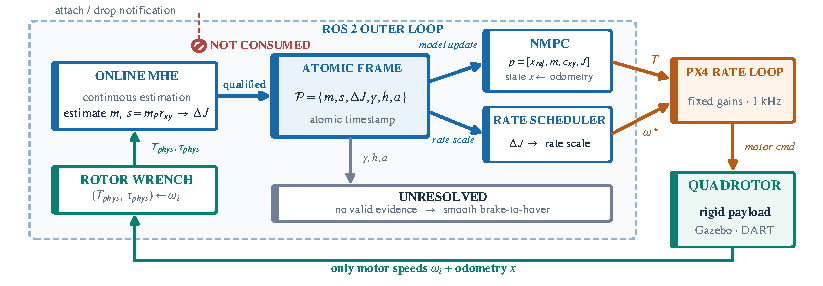
\includegraphics[width=0.98\textwidth]{Figures/fig1_architecture.pdf}
\caption{System architecture and information flow. The complete pipeline consumes
only rotor speeds and odometry. One atomic, health-gated $m/\svec/J$ frame drives
both the NMPC model and the continuous body-rate command scheduling. No
attach or release notification enters this path.}
\label{fig:architecture}
\end{figure}

Two properties of this diagram carry the argument of the dissertation.

First, \textbf{the only inputs are odometry and rotor speeds.} The estimator does
not read the controller's intended thrust or torque
(Section~\ref{sec:model:phys}), does not read the gripper's attach or release
record, and does not read the simulator's joint state. The payload truth
available in simulation is used exclusively for offline scoring.

Second, \textbf{there is exactly one interface.} The estimator publishes a single
atomic frame (Section~\ref{sec:frame:interface}) containing mass, first moment,
the derived geometry, a confidence scalar and a health flag. Both consumers ---
the NMPC model parameters and the inner-loop command scaling --- read that one
frame. An earlier design in which mass, geometry and inertia travelled on
separate topics, each with its own latency and validity, made it possible for the
controller to hold a mutually inconsistent parameter set; the atomic frame makes
that class of fault unrepresentable.

The two optimisers run at different rates and do not share a solve clock. The
estimator solves at \SI{10}{\hertz} over a \SI{2}{\second} window; the controller
solves at \SI{20}{\hertz} over a \SI{1}{\second} preview; setpoints are published
at \SI{50}{\hertz} by interpolating along the most recent predicted trajectory.

\section{Moving Horizon Estimator}\label{sec:frame:mhe}

\subsection{The optimisation}\label{sec:frame:mheocp}

With the augmented state \eqref{eq:xaug} of Chapter~\ref{ch:model}, the estimator
solves, at each \SI{10}{\hertz} tick,
\begin{align}
\min_{x_{0:N},\, w_{0:N-1}} \quad
& \bigl\| x_0 - \bar{x}_0 \bigr\|^2_{W_0}
+ \sum_{j=0}^{N-1} \beta_j \Bigl( \bigl\| y_j - C x_j \bigr\|^2_{W_y}
+ \bigl\| w_j \bigr\|^2_{W_w} \Bigr) \nonumber \\
\mathrm{s.t.} \quad
& x_{j+1} = F_{\mathrm{M}}\bigl(x_j,\, u^{\mathrm{phys}}_j\bigr) + G\,w_j, \nonumber \\
& \underline{m} \le \mT \le \overline{m}, \qquad
  |s_x|,\,|s_y| \le \overline{s},
\label{eq:mhe}
\end{align}
where $y_j$ is the odometry measurement, $C$ selects the thirteen vehicle states
from the sixteen-dimensional augmented state, $F_{\mathrm{M}}$ is one explicit
fourth-order Runge--Kutta step of the dynamics of Chapter~\ref{ch:model} driven
by the reconstructed wrench $u^{\mathrm{phys}}$ of \eqref{eq:phys}, and
\begin{equation}
G = \begin{bmatrix} I_{13} \\ 0_{3\times13}\end{bmatrix}
\label{eq:Gmat}
\end{equation}
confines the process noise to the physical states, leaving $\mT$ and $\svec$
noise-free within the window.

The horizon is $N=20$ stages at $\Delta t=\SI{0.1}{\second}$. The choice is a
compromise that the experiments of Chapter~\ref{ch:evaluation} revisit: a longer
window averages more measurement noise, but the constraint that makes the payload
states identifiable --- that they are \emph{constant} over the window --- becomes
less defensible the longer the arc of trajectory the window spans. On a
\SI{4}{\meter\per\second} figure-eight a ten-stage window recovered the mass
$3.7\times$ more accurately than a twenty-stage one, while a forty-stage window
sat on the lower bound for the entire flight.

\subsection{Weights}\label{sec:frame:weights}

All three weight matrices follow Bryson's rule: each diagonal entry is the
inverse square of a representative magnitude for the corresponding residual, so
that every channel contributes a cost of order unity at its own natural scale and
the Gauss--Newton Hessian is not curvature-imbalanced across directions.

The measurement weight uses representative state-estimation standard deviations,
\begin{equation}
W_y = \mathrm{diag}\Bigl(\sigma_p^{-2}I_3,\ \sigma_v^{-2}I_3,\ \sigma_q^{-2}I_4,\ \sigma_\omega^{-2}I_3\Bigr),
\label{eq:Wy}
\end{equation}
with $\sigma_p=\SI{0.02}{\meter}$, $\sigma_v=\SI{0.05}{\meter\per\second}$,
$\sigma_q=0.01$ (about \SI{1.1}{\degree}) and
$\sigma_\omega=\SI{0.02}{\radian\per\second}$.

The process-noise weight is deliberately \emph{tighter} than the measurement
weight,
\begin{equation}
W_w = \mathrm{diag}\bigl(10^{4} I_6,\ 10^{5} I_4,\ 10^{3} I_3\bigr).
\label{eq:Ww}
\end{equation}
This is the central tuning decision of the estimator, and its rationale is worth
stating explicitly. The purpose of \eqref{eq:mhe} is not to smooth noisy
measurements; it is to force any persistent mismatch between the reconstructed
wrench and the observed motion to be explained by the two payload parameters
rather than absorbed into unstructured process noise. Trusting the dynamics ---
large $W_w$ --- is what makes that attribution happen. The angular block is one
decade looser than the translational block because the rotational equation
contains the gyroscopic product $\bm\omega\times\Jt\bm\omega$ and the inverse
inertia, and is numerically the more delicate of the two.

The arrival cost anchors the start of the window,
\begin{equation}
W_0 = \mathrm{diag}\bigl(10^{3} I_6,\ 10^{4} I_4,\ 10^{2} I_3,\ \sigma_{m,0}^{-2},\ \sigma_{s,0}^{-2}I_2\bigr),
\qquad
\sigma_{m,0} = \SI{3.16}{\kg},\ \ \sigma_{s,0}=\SI{0.1}{\kg\meter},
\label{eq:W0}
\end{equation}
with $\bar x_0$ taken from the previous window's solution shifted forward by one
stage. Two points about the payload entries. First, they are four to five orders
of magnitude softer than the physical-state entries: with
$\sigma_{m,0}=\SI{3.16}{\kg}$ against a vehicle that weighs \SI{2.06}{\kg}
empty, the mass anchor carries essentially no information, and that is
intentional --- it is what allows a payload step to be absorbed within roughly
one window rather than being dragged toward the previous answer. Second, they are
not set to zero. A zero entry removes positive definiteness of the Hessian in
that direction whenever a window happens to be poorly excited, and an earlier
experiment with genuinely uninformative payload channels produced 472 solver
failures from exactly that mechanism. A numerically small but non-zero anchor is
uninformative in the statistical sense while remaining well posed in the
numerical one.

The bounds in \eqref{eq:mhe} are physical rather than tuning knobs. The
composite mass is constrained to
$[\,0.95\,\mB,\ \SI{5.0}{\kg}\,]=[\SI{1.961}{\kg},\SI{5.0}{\kg}]$: the vehicle
cannot weigh less than its own airframe, and the \SI{5}{\percent} margin leaves
room for calibration error rather than pinning the estimate at the calibrated
value. That such a bound is a \emph{hard constraint on a decision variable} is a
concrete advantage of the moving-horizon formulation over a recursive filter,
which can be biased away from non-physical estimates but cannot be forbidden from
producing them. The first moment is bounded loosely,
$\overline{s}=\SI{1.5}{\kg\meter}$, purely to prevent the optimiser from
diverging; the physically meaningful admissibility limit on $\svec$ is applied
later, in the reference-formation logic of Section~\ref{sec:frame:momentref},
where it can reject a sample without distorting the optimisation.

\paragraph{The prior-free ablation.} The lower bound $0.95\,\mB$ and the arrival
mean are the two remaining places where the airframe mass could in principle
inform the mass channel. The implementation therefore retains a switch that
removes both: the bound drops to \SI{0.2}{\kg} --- a value chosen only to keep
$1/\mT$ away from its singularity and containing no airframe information --- and
$\sigma_{m,0}$ rises to \SI{1000}{\kg}. This configuration is an
\emph{ablation}, not the deployed default; the results of
Chapter~\ref{ch:evaluation} are reported under the default unless stated
otherwise. The seed of Section~\ref{sec:model:seed} is prior-free in both
configurations, because it is computed from measurements in either case.

\subsection{Stage weighting: what was tried and what is deployed}\label{sec:frame:beta}

The factors $\beta_j$ in \eqref{eq:mhe} exist because the constant-payload model
is valid on either side of a grasp or release but not across one. When the event
falls inside the current window, a fixed-weight estimator returns a compromise
between two physical regimes until the older regime leaves the horizon --- a
transient on the order of the window length.

Three treatments were implemented and compared.

\paragraph{Event-triggered de-weighting (retired).} The original scheme detected a
persistent step in $\Tphys$ and scaled every stage preceding it by $10^{-4}$,
leaving the arrival cost active so that the physical-state trajectory remained
available as a warm start. On the \SI{2}{\meter\per\second} condition this
schedule remained armed but never fired. At \SI{4}{\meter\per\second} it was
\emph{disabled}, because grasp and release transients are not the only events
that move the collective thrust: a trajectory-mode change produces a step of the
same amplitude, and the detector cannot distinguish them. All results reported in
Chapter~\ref{ch:evaluation} use $\beta_j\equiv1$. A parameterised generalisation
of the schedule was additionally optimised by cross-entropy search, and found no
measurable improvement over the hand-designed rule; that negative result is
substantive, and is discussed in Section~\ref{sec:eval:weightlearning}.

\paragraph{Exponential forgetting (available, off by default).} A continuous
alternative discounts each stage by its age,
\begin{equation}
\beta_j = \lambda^{\,N-1-j}, \qquad j=0 \text{ oldest},
\label{eq:forget}
\end{equation}
giving an effective memory of about $1/(1-\lambda)$ stages --- ten frames
(\SI{1.0}{\second}) at $\lambda=0.9$, five at $\lambda=0.8$. This is the smooth
version of shortening the horizon: it neither changes the problem dimension nor
introduces a new noise channel, and the arrival-cost block is explicitly excluded
from the discount, since that block anchors physical states rather than carrying
stale payload evidence. The deployed default is $\lambda=1$.

\paragraph{Parameter random walk (available, off by default).} The third option
admits process noise on the payload channels themselves, replacing
$\dot{\mT}=0$, $\dot{\svec}=\bm 0$ by a random walk with tuned intensities
$\sigma_{\dot m}$ and $\sigma_{\dot s}$, as is standard in the learned-MHE
literature \cite{neuromhe}. It removes the need for any event logic, since the
parameters can then move within a window. It is off by default because the added
noise channels have natural scales two orders of magnitude apart from the
physical ones, and the resulting Hessian conditioning produced the 472 solver
failures noted above.

The deployed configuration therefore uses no event logic at all. This is a
deliberate simplification and it costs a transient of roughly one window after
each payload change; the lifecycle logic of Section~\ref{sec:frame:lifecycle} is
built to tolerate that transient rather than to shorten it.

\subsection{Re-anchoring and over-range rejection}\label{sec:frame:reanchor}

Two guards protect the estimator from its own failures.

\paragraph{Re-anchoring after repeated solver failure.} After five consecutive
failed solves the window is discarded and rebuilt: the physical states are reset
to the current measurement, the mass is re-seeded from \eqref{eq:winbal}, and
$\svec$ is reset to zero. The choice of zero is not neutral --- it asserts ``no
payload'' --- and it therefore has a consequence that the release logic must
respect: a first moment that is zero \emph{because the window was just rebuilt}
is not evidence of a release. Section~\ref{sec:frame:decision} states that rule
explicitly.

\paragraph{Physically inadmissible first moments.} The platform cannot realise a
first moment larger than
\begin{equation}
\lVert\svec\rVert_{\max} = \mP^{\mathrm{env}}\, r_{xy}^{\max}
= \SI{0.30}{\kg}\times\SI{0.13}{\meter} = \SI{0.039}{\kg\meter},
\label{eq:sadmissible}
\end{equation}
so a solved $\lVert\hat\svec\rVert$ above that bound is a statement about the
estimator, not about the payload. Such samples are excluded from the
reference-formation window of Section~\ref{sec:frame:momentref} and counted as an
estimator-quality diagnostic; if they persist while the vehicle is not
manoeuvring, the window is re-anchored. They are \emph{not} removed from the
published frame, which is a limitation recorded in Chapter~\ref{ch:evaluation}:
an out-of-envelope $\hat\svec$ still reaches the controller's $\cvec$ through the
filter and slew limiter.

\section{The Continuous Payload Interface}\label{sec:frame:interface}

\subsection{One atomic frame}\label{sec:frame:frame}

After each solve the estimator publishes
\begin{equation}
\mathcal{P} = \Bigl\{\, \mT,\; s_x, s_y,\; c_x, c_y,\;
\dJ_{xx},\dJ_{yy},\dJ_{zz},\; J_{xx},J_{yy},J_{zz},\; \gamma,\; h,\; a \,\Bigr\},
\label{eq:frame}
\end{equation}
in which the geometry entries are computed from $(\mT,\svec)$ by
\eqref{eq:c_from_s} and \eqref{eq:Jdeployed}, $\gamma\in[0,1]$ is the no-payload
confidence of Section~\ref{sec:frame:gamma}, $h$ is a health bit and $a$ is the
age of the most recent successful solution.

Health is a conjunction: the latest solve must have succeeded, and the odometry,
rotor-speed and known-input streams must all be fresher than
\SI{0.30}{\second}. The consumer applies one further test of its own, on the
receive age of the frame itself (\SI{0.35}{\second}), because a frame can be
healthy at the moment it is produced and stale by the time it is used.

The asymmetry in how an unhealthy frame is treated is deliberate and is the
safety property of the interface: \emph{an unhealthy or stale frame freezes the
last accepted model and resets the confidence persistence timer}. A degraded
estimate can therefore delay a release confirmation, but it can never cause one.

\subsection{Filtering and slew limiting}\label{sec:frame:filter}

A valid frame is not consumed directly. Each channel passes a first-order
low-pass filter and a separate rate limiter before it reaches the solver:
\begin{equation}
\alpha = 1 - e^{-\Delta t/\tau},
\qquad
\hat\theta \;\leftarrow\; \hat\theta + \alpha\bigl(\theta^{\mathrm{tgt}} - \hat\theta\bigr),
\qquad
\hat\theta \;\leftarrow\; \hat\theta + \mathrm{clip}\bigl(\cdot,\ \pm \dot\theta_{\max}\Delta t\bigr),
\label{eq:lpfslew}
\end{equation}
with $\tau=\SI{0.20}{\second}$ on the controller side
($\SI{0.25}{\second}$ on the estimator's own output stage) and rate limits
$\SI{0.60}{\kg\per\second}$ for the mass, $\SI{0.080}{\kg\meter\per\second}$ for
the first moment and $\SI{0.080}{\kg\meter\squared\per\second}$ for the inertia
increment.

The reason for a limiter in addition to a filter is that the two protect against
different things. The filter attenuates noise; the limiter bounds how fast the
\emph{model} underneath a receding-horizon optimisation may change. A parameter
step between consecutive solves invalidates the warm start, and an optimiser that
must re-converge from scratch at \SI{20}{\hertz} is an optimiser that
occasionally does not converge in time. The limiter converts any step ---
including a genuine one at grasp --- into a ramp the solver can track.

\section{The Eventless Grasp--Release Lifecycle}\label{sec:frame:lifecycle}

\subsection{Why refuse the command}\label{sec:frame:why-eventless}

The controller in this work issues the gripper-release command itself. It would
be trivial to clear the payload model at that instant, and every command-triggered
implementation does so. The reason not to is that a release command is a
\emph{request}, and the model must describe the \emph{vehicle}.

The two diverge in practice. A gripper can be slow to open, can jam, can release
only part of a multi-item load, or can release nothing at all; conversely, a load
can be torn off, can slip, or can be released by an agent whose notification
never arrives. In each case a command-triggered controller flies a loaded vehicle
with an empty model, or an empty vehicle with a loaded one. The failure is silent,
because nothing in the control loop contradicts it.

The eventless alternative accepts a cost --- confirmation is delayed by the time
the estimator needs to accumulate evidence --- in exchange for a model that is
never wrong for a reason the vehicle cannot detect.
Chapter~\ref{ch:evaluation} measures both sides of that trade.

\subsection{Two state machines}\label{sec:frame:fsm}

The lifecycle is split between the two nodes, as shown in
Figure~\ref{fig:fsm}. The estimator owns payload \emph{presence} and may
\emph{declare} a release. The controller owns the payload \emph{model} and clears
it only on \emph{confirmation}. Declaration is neither necessary nor sufficient
for confirmation; the separation exists so that a single detector cannot, by
itself, empty the controller's model.

\begin{figure}[ht]
\centering
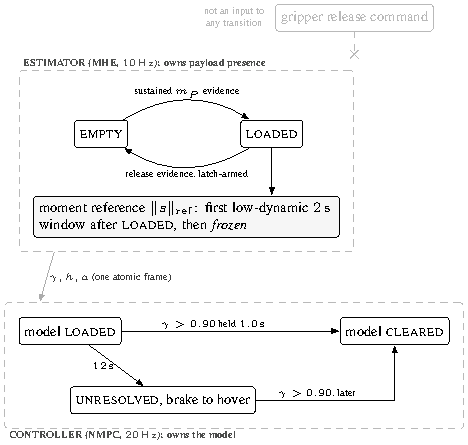
\includegraphics[width=0.92\textwidth]{Figures/fig_lifecycle_fsm.pdf}
\caption{The payload lifecycle as two state machines. The estimator owns payload
presence and may declare release from the evidence of
\eqref{eq:release-evidence}; the controller owns the model and clears it only on
confirmation, $\gamma>0.90$ held for \SI{1.0}{\second}. The gripper release
command enters neither machine. \textsc{unresolved} is a hold, not a clearing:
the model stays loaded while the vehicle brakes to hover and keeps waiting for
evidence.}
\label{fig:fsm}
\end{figure}

Presence is a hysteretic \textsc{empty}$\leftrightarrow$\textsc{loaded} machine
driven by sustained payload-mass evidence, with a directional thrust residual as
a fast path into \textsc{loaded}. A separate latch records that the present
flight reliably entered \textsc{loaded} at some point. That latch does two jobs:
it prevents an empty-flight confidence value from consuming the later release
confirmation, and it prevents a transient mass dip during the figure-eight from
disarming the true release path.

\subsection{No-payload confidence}\label{sec:frame:gamma}

Every lifecycle decision is a function of the published frame \eqref{eq:frame}
alone. The confidence scalar $\gamma$ fuses three ``empty'' indications.

Let $\sigma(v;a,b)$ be the smooth indicator that is $1$ for $|v|\le a$, $0$ for
$|v|\ge b$, and in between
\begin{equation}
\sigma(v;a,b) = 1 - \bigl(3\chi^2 - 2\chi^3\bigr),
\qquad \chi = \frac{|v|-a}{b-a},
\label{eq:smoothstep}
\end{equation}
which is the standard cubic smooth-step: continuous with continuous first
derivative at both ends, so $\gamma$ cannot jump when a channel crosses a
threshold. Then
\begin{equation}
\gamma \;=\; \sigma\bigl(\mP;\,0.015,\,0.060\bigr)\;\cdot\;
             \sigma\bigl(\lVert\svec\rVert;\,0.0015,\,0.0060\bigr)\;\cdot\;
             \sigma\bigl(\dJ_{xy};\,0.0020,\,0.0100\bigr),
\label{eq:gamma}
\end{equation}
with thresholds in \si{\kg}, \si{\kg\meter} and \si{\kg\meter\squared}, and
$\dJ_{xy}=\max(|\dJ_{xx}|,|\dJ_{yy}|)$.

The choice of a \emph{product} rather than a sum or a vote is deliberate: any
single payload indication vetoes \textsc{empty}. In particular a non-zero first
moment keeps $\gamma$ low even when the scalar mass estimate happens to be
sitting on its lower bound --- which, as Section~\ref{sec:model:whyS} showed, is
exactly the state the predecessor design entered after a release. The product
turns that failure mode into a refusal to confirm rather than a false
confirmation.

It is worth being precise that \eqref{eq:gamma} is a \emph{state-quality} metric
for a payload that has already gone, not a transition detector. The moment factor
carries an absolute threshold, and a state transition must not depend on the
estimator's noise floor happening to lie below an absolute number. The release
detector of Section~\ref{sec:frame:decision} therefore uses the individual
indications, not their product.

\subsection{The loaded moment reference}\label{sec:frame:momentref}

The release detector is built on a \emph{ratio},
\begin{equation}
\rho \;=\; \frac{\lVert\svec\rVert}{\sref},
\label{eq:rho}
\end{equation}
and the reason is empirical. Over five development flights the loaded and
released distributions of $\lVert\svec\rVert$ \emph{overlap}: the loaded minimum,
\SI{0.0039}{\kg\meter}, lies below the released maximum,
\SI{0.0049}{\kg\meter}. No absolute threshold separates them. The ratio does,
because it compares the vehicle against itself.

That requires a reference the estimator must form autonomously. A running maximum
is not acceptable --- it would absorb precisely the figure-eight estimation
errors the detector exists to reject, and \SIrange{7.6}{18.3}{\percent} of loaded
frames exceed the physical bound \eqref{eq:sadmissible} during the manoeuvre,
which would depress the denominator until $\rho$ crossed its threshold with the
payload still attached. The deployed procedure instead forms a reference once and
freezes it:

\begin{enumerate}
\item \textbf{Admissibility.} After the \textsc{loaded} declaration, a healthy
frame is admitted only if $\lVert\hat\svec\rVert\le\SI{0.039}{\kg\meter}$ by
\eqref{eq:sadmissible}. An out-of-envelope sample is discarded, not clipped:
clipping would still build the denominator from a sample known to be wrong.

\item \textbf{Low dynamics.} The vehicle must satisfy
$\lVert\bm\omega\rVert\le\SI{0.15}{\radian\per\second}$ and
$\lVert\bm v_{xy}\rVert\le\SI{0.20}{\meter\per\second}$. This is an
\emph{online} criterion, not ``wait $N$ seconds after grasp'': the latter would
only be correct for one particular mission script.

\item \textbf{Persistence.} Twenty consecutive admitted frames
(\SI{2}{\second}) must accumulate; any manoeuvre clears the buffer.

\item \textbf{Magnitude stability.} The window must satisfy
\begin{equation}
\frac{1.4826\cdot\mathrm{MAD}\bigl(\lVert\svec_j\rVert\bigr)}
     {\mathrm{median}\bigl(\lVert\svec_j\rVert\bigr)} \;\le\; 0.25,
\label{eq:madcv}
\end{equation}
where the factor $1.4826$ converts the median absolute deviation into a
consistent estimate of the standard deviation for Gaussian data. A robust
dispersion measure is used rather than the sample standard deviation because a
single outlying frame must not be able to veto an otherwise clean window.

\item \textbf{Direction consistency.} The window must further satisfy
\begin{equation}
\Bigl\lVert \frac{1}{20}\sum_{j} \frac{\svec_j}{\lVert\svec_j\rVert} \Bigr\rVert \;\ge\; 0.90 ,
\label{eq:dirmean}
\end{equation}
that is, the mean \emph{unit} first-moment vector must be close to unit length.
This catches the failure mode that \eqref{eq:madcv} cannot: a sequence whose
magnitude is perfectly steady while its direction rotates or flips sign frame to
frame, which is the signature of an ill-conditioned rotational channel rather
than of a real eccentric load.

\item \textbf{Robust statistic and freeze.} The reference is the
\SI{20}{\percent}-trimmed mean of the window magnitudes, and it is frozen for the
remainder of the flight.
\end{enumerate}

If no window qualifies before the vehicle enters the aggressive segment, $\rho$
never becomes available and the moment-gated path cannot fire. That is a genuine
miss mode, and it is the dominant one in the results of
Chapter~\ref{ch:evaluation}.

\subsection{Release evidence and the decision rule}\label{sec:frame:decision}

The detector organises its inputs into three \emph{independent} information
sources. The word is used strictly: an earlier version counted the mass channel
and the inertia channel as two votes, which was false robustness, since in the
continuous interface $\dJ=A(\mP)$ is a deterministic function of the mass and the
fixed $r_z$. They carry one piece of evidence, not two.

\begin{equation}
\begin{aligned}
\text{moment collapse}\quad&:\quad \rho < 0.30 \ \wedge\ \lVert\svec\rVert < \SI{0.008}{\kg\meter},\\
\text{quantity empty}\quad&:\quad \mP < \SI{0.030}{\kg},\\
\text{residual drop}\quad&:\quad \text{a signed thrust step, Section~\ref{sec:frame:resid}.}
\end{aligned}
\label{eq:release-evidence}
\end{equation}
The absolute bound in the first line is a sanity limit, not a discriminator ---
the distributions overlap, as noted above --- and it exists only to reject the
case in which an anomalously large reference peak makes $\rho$ spuriously small.

The decision rule is then
\begin{equation}
\text{release} \;\Longleftrightarrow\; \text{armed} \ \wedge\ \bigl[\, \text{slow path} \ \vee\ \text{fast path} \,\bigr],
\label{eq:releasedecision}
\end{equation}
in which
\begin{equation}
\begin{aligned}
\text{slow path}\;:\quad & \text{quantity empty} \ \wedge\ \text{moment collapse},
  \ \text{sustained } 5 \text{ frames},\\
\text{fast path}\;:\quad & \text{strong residual} \ \wedge\ \text{moment collapse},
  \ \text{sustained } 4 \text{ frames},
\end{aligned}
\label{eq:releasepaths}
\end{equation}
where \emph{armed} records that the present flight reliably entered
\textsc{loaded} at some earlier point.

\textbf{Moment evidence is mandatory in both paths}, and the reason is a recorded
failure. An earlier rule admitted a third path --- residual together with
quantity-empty, without moment evidence --- and it released prematurely in 3 of 9
randomised flights, the earliest \SI{51.1}{\second} before the release command.
Its design assumption, that ``quantity empty is false while the payload is
attached'', is simply untrue at \SI{4}{\meter\per\second}: the mass estimate sits
on its lower bound for whole stretches of a figure-eight, so $\mP$ is
persistently below \SI{0.03}{\kg} for a median of \SI{14}{\second} and as long as
\SI{48}{\second} in loaded flight. Neither amplitude nor persistence separates
that from a real release. The plain residual vote is likewise false-positive
during manoeuvre. The discarded path was therefore two unreliable channels
conjoined, with nothing able to veto them. The moment channel is the one that
measured cleanly: across those same flights the loaded $\rho$ bottomed at
$0.789$ against a threshold of $0.30$, a factor of $2.6$ of margin, with zero
false positives.

The cost of making moment evidence mandatory is accepted explicitly: \emph{a
release whose $\rho$ never collapses is not detected here.} That is a miss, and
it is handled by the \textsc{unresolved} path of
Section~\ref{sec:frame:unresolved} --- never by releasing on weaker evidence.

Two further rules close known loopholes. First, moment evidence must come from a
fresh, successful solve: the re-anchoring of Section~\ref{sec:frame:reanchor}
initialises $\svec$ to zero, and that zero is not counted as a collapse. Second,
the online and offline evaluations call the same pure decision function, so a
replay of a recorded flight exercises exactly the deployed logic rather than a
re-implementation of it.

\subsection{The release-residual vote}\label{sec:frame:resid}

The residual channel compares two adjacent half-windows of the reconstructed
collective thrust,
\begin{equation}
\Delta T_k \;=\; \overline{T}_{\mathrm{post}} - \overline{T}_{\mathrm{pre}}
\;=\; \frac{1}{h}\sum_{i=k-h+1}^{k} T^{\mathrm{phys}}_{i}
\;-\; \frac{1}{h}\sum_{i=k-2h+1}^{k-h} T^{\mathrm{phys}}_{i} ,
\qquad h=3 ,
\label{eq:deltaT}
\end{equation}
that is, two \SI{0.3}{\second} means at \SI{10}{\hertz}. A release makes
$\Delta T$ negative, because the vehicle no longer supports the load.

Amplitude alone is not enough: a recorded figure-eight transient reached
\SI{-1.69}{\newton}, which is larger in magnitude than the \SI{-1.47}{\newton}
weight of the smallest payload tested. The vote therefore combines a floor with a
robust significance test against the recent history of $\Delta T$ itself,
\begin{equation}
\hat\sigma_{\Delta T} = \max\Bigl(1.4826\cdot\mathrm{MAD}\bigl(\{\Delta T_i\}_{i<k}\bigr),\ \SI{0.05}{\newton}\Bigr),
\qquad
z_k = \frac{-\Delta T_k}{\hat\sigma_{\Delta T}} ,
\label{eq:deltaTz}
\end{equation}
where the history deliberately excludes the current frame, since a step included
in its own dispersion estimate inflates $\hat\sigma$ and hides itself. A vote is
cast when $\Delta T_k<\SI{-0.9}{\newton}$ persists for two frames, and a
\emph{strong} vote --- the one eligible to pair with a moment collapse in
\eqref{eq:releasedecision} --- when it persists for four.

Residual votes are \emph{edge} events and are given an explicit validity window
of \SI{3}{\second}. A vote that has expired is no longer evidence. This is a
small detail with a large consequence: without it, a single manoeuvre transient
early in a flight would remain available to be combined with an unrelated moment
collapse minutes later.

\subsection{Confirmation, \textsc{unresolved}, and braking to hover}\label{sec:frame:unresolved}

The controller clears its payload model through exactly one route:
\begin{equation}
\gamma > 0.90 \quad\text{held for}\quad \SI{1.0}{\second}
\quad\text{on healthy, fresh frames.}
\label{eq:confirm}
\end{equation}
An estimator declaration accelerates this but does not bypass it. On accepted
release evidence the estimator switches only the \emph{published target} of
$\svec$ to zero; the optimisation state is not overwritten. The output filter of
\eqref{eq:lpfslew} consequently produces a continuous decay rather than a
geometric step, and $\gamma$ rises smoothly through \eqref{eq:gamma}.
Confirmation can also occur with no declaration at all, driven by the estimator
converging on its own; the moment factor in \eqref{eq:gamma} still vetoes it
while $\lVert\svec\rVert$ is non-zero.

If no confirmation arrives within \SI{12}{\second} of the release command, the
controller enters \textsc{unresolved}. This state is the reason the eventless
design is deployable, and its semantics deserve emphasis: \textbf{a timeout is
not a release}. The model stays loaded. What changes is the vehicle's exposure:
it stops flying an aggressive trajectory it may no longer have the authority to
fly, and it gives the estimator a quiet operating point in which
Section~\ref{sec:frame:momentref}'s low-dynamic criterion can finally be met.

The braking manoeuvre is a finite-time reference rather than an instantaneous
switch to hover, because at \SI{4}{\meter\per\second} the latter would command a
step of several metres per second. Let $\bm p_0,\bm v_0$ be the state at the
declaration and $T_b=\SI{3}{\second}$. The stopping point is chosen as the
displacement of a constant deceleration from $\bm v_0$ to rest,
\begin{equation}
\bm p_1 = \bm p_0 + \tfrac{1}{2} T_b\, \bm v_0 ,
\label{eq:brakep1}
\end{equation}
and the reference between the two is the unique quintic satisfying
$\bm p(0)=\bm p_0$, $\dot{\bm p}(0)=\bm v_0$, $\ddot{\bm p}(0)=\bm 0$,
$\bm p(T_b)=\bm p_1$, $\dot{\bm p}(T_b)=\bm 0$, $\ddot{\bm p}(T_b)=\bm 0$:
\begin{equation}
\bm p(t) = \bm p_0 + \bm v_0 t + a_3 t^3 + a_4 t^4 + a_5 t^5,
\qquad
\begin{aligned}
a_3 &= \bigl(10\,\Delta\bm p - 6 T_b \bm v_0\bigr)/T_b^3,\\
a_4 &= \bigl(-15\,\Delta\bm p + 8 T_b \bm v_0\bigr)/T_b^4,\\
a_5 &= \bigl(6\,\Delta\bm p - 3 T_b \bm v_0\bigr)/T_b^5,
\end{aligned}
\label{eq:quintic}
\end{equation}
with $\Delta\bm p=\bm p_1-\bm p_0$. Zero acceleration at both ends means the
manoeuvre begins and ends without a jump in commanded thrust, which is what
keeps the transition from itself perturbing the estimator whose evidence is being
awaited. Attitude is blended over the same interval by the smooth-step of
\eqref{eq:smoothstep}.

\subsection{Threshold provenance}\label{sec:frame:thresholds}

Table~\ref{tab:thresholds} lists every lifecycle threshold and where its value
came from. All were fixed in code before the final campaign began and were not
retuned on it. Only the ratio threshold and the residual floor were selected
against data, and that data is from earlier flights that are disjoint from the
reported campaign; the remainder are engineering choices whose closed-loop
sensitivity has not been swept, and are reported as such.

\begin{table}[ht]
\centering
\caption{Lifecycle thresholds and their provenance. ``Earlier flights'' predate,
and are disjoint from, the reported campaign.}
\label{tab:thresholds}
\small
\begin{tabularx}{\textwidth}{@{}p{0.26\textwidth} p{0.20\textwidth} X@{}}
\toprule
\textbf{Threshold} & \textbf{Value} & \textbf{Provenance} \\
\midrule
moment-collapse ratio $\rho$ & $0.30$ &
leave-one-out cross-validation on 59 earlier flights; every fold selected
$0.30$, whereas $0.20$ succeeded in only 48 of 59 \\
residual floor / persistence & \SI{0.9}{\newton}; 2 or 4 frames &
below the \SI{1.47}{\newton} weight of the smallest payload; on a recorded
flight, figure-eight excursions past \SI{0.9}{\newton} lasted at most three
frames while the release step lasted four \\
slow-path persistence & 5 frames (\SI{0.5}{\second}) & engineering choice \\
mass-domain release & $\mP<\SI{0.030}{\kg}$, 20 frames &
between the loaded minimum (\SI{0.079}{\kg}) and the post-release maximum
(\SI{0.007}{\kg}) of earlier \SI{0.15}{\kg} flights \\
no-payload confidence & $0.90$ held \SI{1.0}{\second} & engineering choice \\
reference window & 20 frames; $\mathrm{CV}\le0.25$; direction $\ge0.90$ & engineering choice \\
\textsc{unresolved} timeout / brake & \SI{12}{\second} / \SI{3}{\second} & engineering choice \\
\bottomrule
\end{tabularx}
\end{table}

\section{Adaptive NMPC}\label{sec:frame:nmpc}

\subsection{Cost and weights}\label{sec:frame:nmpcweights}

The controller solves \eqref{eq:nmpc} with $N=20$ stages at
$\Delta t=\SI{0.05}{\second}$, preserving a \SI{1.0}{\second} preview while
running at \SI{20}{\hertz}. The residual vector is
\begin{equation}
\begin{aligned}
y_k = \bigl[\, &\bm e_p;\ \bm e_v;\ \bm e_{q,\mathrm{vec}};\ \bm e_\omega;\\
&u_k - u_{\mathrm{hover}}(p) \,\bigr] \in \mathbb{R}^{16},
\end{aligned}
\label{eq:nmpcresidual}
\end{equation}
where the attitude entry is the vector part of the relative quaternion
$\bm q_{\mathrm{ref}}^{*}\otimes\bm q$, which keeps the residual on the tangent
space of the rotation manifold instead of treating four quaternion components as
independent Euclidean coordinates.

Weights again follow Bryson's rule, $Q_{ii}=L_i^{-2}$, with tolerances
\begin{equation}
L_p=\SI{0.1}{\meter},\quad
L_v=\SI{0.3}{\meter\per\second},\quad
L_q=0.05,\quad
L_\omega=\SI{0.3}{\radian\per\second},
\label{eq:Lstate}
\end{equation}
and, on the inputs,
$L_T=\SI{2}{\newton}$, $L_{\tau,xy}=\SI{0.5}{\newton\meter}$,
$L_{\tau,z}=\SI{0.2}{\newton\meter}$; the torque scales are taken to be the
constraint bounds themselves, since the input cannot exceed them in any case. The
terminal weight rescales the stage blocks by $20$ (position), $1$ (velocity), $2$
(attitude) and $0.2$ (rate): the endpoint of the prediction is pulled tightly
onto the reference in position and attitude, while relaxing the terminal rate
demonstrably helps the solver.

This non-dimensionalisation is not cosmetic. Before it was applied, position and
torque weights differed by a factor of tens at their natural magnitudes, the
Gauss--Newton Hessian was correspondingly ill-conditioned across directions, and
the stationarity residual was observed to reach $6.26\times10^{5}$ --- a complete
numerical breakdown rather than a slow convergence.

\paragraph{Trajectory-scaled tolerances.} Two of the entries in \eqref{eq:Lstate}
are defined by the comment that accompanies them as trajectory-dependent
quantities: $L_v$ is a characteristic speed and $L_\omega$ a characteristic yaw
rate. Written as constants they are correct only for the low-speed reference they
were tuned on. An optional rescaling restores the intent,
\begin{equation}
L_v \leftarrow \max\bigl(L_v,\ r\,w\bigr),
\qquad
L_\omega \leftarrow \max\bigl(L_\omega,\ K_\psi\, w\bigr),
\qquad K_\psi = 3.17,
\label{eq:trajscale}
\end{equation}
taking the maximum so that the weights are only ever relaxed, never tightened.
The constant $K_\psi$ is the ratio of peak yaw rate to angular rate on the
figure-eight of Section~\ref{sec:frame:ref}, obtained numerically; it is worth
noting that evaluating the yaw rate at the intuitive location $a=\pi/4$ gives
$2.83$ and underestimates the peak by \SI{12}{\percent}, because the extremum
does not occur there. Applying \eqref{eq:trajscale} at the low-speed condition
reproduces $L_v$ exactly but relaxes $L_\omega$ by a factor of $3.2$, which
exposes a pre-existing mismatch rather than introducing one: the original value
was documented as matching a \emph{circular} trajectory, whose yaw rate is
constant at $w$, while the vehicle actually flies a figure-eight whose peak is
$3.17w$. The rescaling is off by default so that historical batches remain
reproducible.

\subsection{Solver}\label{sec:frame:solver}

Both optimal control problems are transcribed by direct multiple shooting with
explicit fourth-order Runge--Kutta integration, a Gauss--Newton Hessian
approximation, and partial-condensing HPIPM \cite{hpipm} as the quadratic
subproblem solver, generated and solved with acados \cite{acados}. Both use
\emph{full} sequential quadratic programming with merit-function backtracking
rather than the real-time-iteration scheme \cite{diehl2005rti}: RTI was observed
to diverge silently in this configuration, and a controller that reports success
while producing a diverging input is worse than one that takes an extra
millisecond. Generated C code is cached and reused until the model or problem
dimensions change.

\section{Inner-Loop Scheduling}\label{sec:frame:omegascale}

\subsection{From inertia ratio to a command scale}\label{sec:frame:scale}

Section~\ref{sec:model:gain} established that a five-fold inertia increase costs
the autopilot's rate loop most of its bandwidth, and that the outer loop cannot
recover it by being more accurate. The deployed response scales the body-rate
\emph{command} around the current measured rate,
\begin{equation}
\bm\omega_{\mathrm{cmd}}' \;=\; \bm\omega \;+\; \varsigma\,\bigl(\bm\omega_{\mathrm{cmd}} - \bm\omega\bigr),
\qquad \varsigma \ge 1,
\label{eq:omegascale}
\end{equation}
applied to the roll and pitch channels only, since $\dJ$ enters only $J_{xx}$ and
$J_{yy}$. Equation~\eqref{eq:omegascale} exaggerates the rate \emph{error} the
inner loop sees, which is equivalent to raising its proportional gain, without
modifying any autopilot parameter. Because it is a common scale on the roll/pitch
pair it preserves the direction of the rate-error vector.

The requested scale is the inertia ratio \eqref{eq:gain}, clipped at a cap of
$5.0$, evaluated from the live $\dJ$ of the payload frame. Three filters stand
between the request and its application, each addressing a distinct failure:

\begin{itemize}
\item a \textbf{dead band} of $0.08$ on the target, so that estimator noise
cannot move it, with explicit snapping to $1.0$ and to the cap so that hysteresis
cannot strand the empty-airframe steady state permanently above unity;
\item a \textbf{first-order filter} with $\tau=\SI{0.5}{\second}$, chosen far
slower than the inner loop (hundreds of hertz) and still fast enough to follow the
second-scale progressive load transfer during a grasp;
\item \textbf{asymmetric rate limits}, \SI{4.0}{\per\second} rising against
\SI{1.5}{\per\second} recovering, encoding the asymmetry of the consequences:
being late to add authority risks saturation, being late to remove it does not.
\end{itemize}

\subsection{Headroom limiting}\label{sec:frame:headroom}

Scaling a command that is already close to the rate limit accomplishes nothing
except saturation, at which point the scaling has silently stopped acting. The
implementation therefore solves for the largest scale that keeps the scaled
command inside a guard band $\pm L$, with $L$ equal to \SI{95}{\percent} of the
hard rate limit $\overline{\omega}=\SI{2.0}{\radian\per\second}$.

For one channel, write the rate error $e=\omega_{\mathrm{cmd}}-\omega$. Requiring
$|\omega+\varsigma e|\le L$ gives
\begin{equation}
\varsigma \;\le\;
\begin{cases}
\dfrac{L-\omega}{e}, & e>0,\\[8pt]
\dfrac{-L-\omega}{e}, & e<0,
\end{cases}
\label{eq:headroom}
\end{equation}
and the applied scale is the smallest such bound over the roll and pitch
channels, floored at unity:
\begin{equation}
\varsigma_{\mathrm{eff}} = \max\Bigl(1,\ \min_{i\in\{x,y\}} \varsigma_i^{\max}\Bigr).
\label{eq:headroomapply}
\end{equation}
The floor at unity guarantees that the scheduler can never make the raw
controller command \emph{less} authoritative than it would have been without
scheduling --- the scheduler is allowed to help and not allowed to hurt. When
\eqref{eq:headroomapply} binds, it is logged, so that saturation avoidance is an
observable event rather than a silent degradation.

\subsection{Attach-time inertia bootstrap}\label{sec:frame:bootstrap}

One interval resists the eventless principle: the second or so between a load
beginning to take weight and the estimator accumulating enough evidence to say
so. During that interval the vehicle is physically loaded and the model is not,
and it is the interval in which the predecessor implementation lost eleven of
sixteen flights at the heaviest condition.

The deployed bootstrap addresses it with the narrowest intervention that works.
At the start of lift, the \emph{inertia} parameter alone is floored at the value
implied by the platform's \SI{0.30}{\kg} payload envelope; mass and first moment
are untouched, and no payload is fabricated in either. The overlay is then faded
out over \SI{0.5}{\second} once the estimator independently reports persistent
loaded evidence, namely $\dJ\ge\SI{0.010}{\kg\meter\squared}$ together with a
confidence well below the confirmation threshold, sustained for
\SI{0.5}{\second}. If the estimate becomes stale or unhealthy while the handover
is in progress, the fade freezes at the last safe inertia rather than continuing
toward zero.

Three properties keep this consistent with the rest of the design. It is
\emph{inertia-only}, so it cannot influence the mass or moment channels on which
every release decision depends. It is \emph{one-directional}, active only at
attach, so the release path remains estimate-only. And its magnitude is the
airframe's payload envelope, which Section~\ref{sec:model:whynot} has already
disclosed as a platform specification rather than task information.

\section{Reference Trajectory}\label{sec:frame:ref}

The evaluation trajectory is a three-dimensional Gerono lemniscate,
\begin{equation}
x_r = r\sin a, \qquad
y_r = r\sin a\cos a = \tfrac{r}{2}\sin 2a, \qquad
z_r = z_h + d_z\sin a, \qquad a = w\,t_c ,
\label{eq:fig8}
\end{equation}
with yaw commanded along the velocity vector. This curve is chosen because its
self-intersection is well behaved: differentiating \eqref{eq:fig8} gives
$\bm v = rw(\cos a,\ \cos 2a)$, whose magnitude at the crossing $a\in\{0,\pi\}$
is $\sqrt2\,rw\neq0$, while both acceleration components are proportional to
$\sin a$ or $\sin 2a$ and vanish there. The velocity therefore does not reverse
and the curvature does not blow up --- it is not a cusp --- yet the yaw must turn
substantially faster through the crossing than on a circle of the same speed,
which is precisely the coupling the evaluation wants. The vertical term gives the
two lobes different heights, increasing coupling while keeping the workspace
compact.

Amplitude is grown from zero after an initial hover by the quintic smooth step
$\alpha(s) = 10s^3-15s^4+6s^5$, which has zero first and second derivative at
both ends. The ramp duration is not arbitrary. The velocity during the ramp is
$\dot\alpha\,(x_f-x_0) + \alpha\,\dot x_f$; requiring the extra term contributed
by the amplitude growth to stay below half the trajectory's own characteristic
speed gives
\begin{equation}
\frac{1.875\,r}{t_{\mathrm{ramp}}} \le \tfrac{1}{2}\sqrt{2}\,r\,w
\qquad\Longrightarrow\qquad
t_{\mathrm{ramp}} \ge \frac{2.65}{w},
\label{eq:ramp}
\end{equation}
where $1.875/t_{\mathrm{ramp}}$ is the peak of $\dot\alpha$. The radius cancels:
how long a ramp is needed depends only on the angular rate, not on the size of
the figure.

\section{Online Execution Sequence}\label{sec:frame:sequence}

At every control instant the implementation performs the following sequence.

\begin{enumerate}
\item Receive and frame-convert the latest odometry.
\item Reconstruct the physical wrench from rotor speeds, \eqref{eq:phys},
averaging the \SI{250}{\hertz} samples over the estimation interval.
\item Append the measurement and the reconstructed input to the \SI{10}{\hertz}
window; re-seed by \eqref{eq:winbal} if the window must be rebuilt.
\item Solve \eqref{eq:mhe} for $(\mT,\svec)$ and the physical trajectory.
\item Update the presence machine, the frozen moment reference
(Section~\ref{sec:frame:momentref}) and the residual vote
(Section~\ref{sec:frame:resid}); evaluate the release decision
\eqref{eq:releasedecision}.
\item Assemble and publish the atomic frame \eqref{eq:frame} with its health bit
and solution age.
\item In the controller: validate freshness, low-pass filter and slew-limit the
frame \eqref{eq:lpfslew}, and write $\mT$, $\dJ$ and $\cvec=\svec/\mT$ into the
model parameters and the hover baseline \eqref{eq:hover}.
\item Evaluate confirmation \eqref{eq:confirm} and the \textsc{unresolved}
timeout; switch the reference to the braking quintic \eqref{eq:quintic} if the
timeout expires.
\item Shift the previous solution forward as a warm start, solve
\eqref{eq:nmpc}, and publish the first input; invert thrust to throttle by
\eqref{eq:throttleinv} and apply the body-rate scaling
\eqref{eq:omegascale}--\eqref{eq:headroomapply}.
\item Log estimates, residuals, constraint activity, solver statistics and every
lifecycle transition.
\end{enumerate}

Estimator and controller failures are handled separately and asymmetrically. An
invalid estimator solve retains the last accepted parameter set and marks the
frame unhealthy, which --- by Section~\ref{sec:frame:frame} --- freezes the
controller's model and resets its confirmation timer. An invalid controller solve
falls back to the configured safe action rather than publishing an unconstrained
command.

\end{spacing}
\newpage

%=== CHAPTER FIVE ===
%% Implementation and experimental evaluation.  Rewritten 2026-09-18 against the
%% frozen SITL campaign of the deployed eventless interface.

\chapter{Implementation and Experimental Evaluation}
\label{ch:evaluation}
\begin{spacing}{1.5}
\setlength{\parskip}{0.22in}

\section{Software-in-the-Loop Platform}\label{sec:eval:platform}

The implementation is organised as ROS~2 packages around PX4
software-in-the-loop \cite{px4} and Gazebo \cite{gazebo}. The controller node
owns the reference generator, the predictive optimal control problem, the mission
sequence and the release-confirmation logic; the estimator node owns the sliding
measurement window, the physical-input reconstruction, the payload-state
optimisation, the lifecycle detector and the published payload frame. The two
communicate through the single atomic frame of
Section~\ref{sec:frame:interface}.

\begin{table}[ht]
\centering
\caption{Main implementation components of the deployed pipeline.}
\label{tab:software}
\small
\begin{tabularx}{\textwidth}{@{}l X X@{}}
\toprule
\textbf{Component} & \textbf{Role} & \textbf{Principal signals} \\
\midrule
Gazebo (Harmonic) & Rigid-body physics; detachable-joint gripper &
pose, rotor speed, attach/detach record (logging only) \\
PX4 SITL & State estimation, rate loop, control allocation &
odometry, actuator commands \\
\texttt{mhe\_node} & 16-state moving-horizon estimation; lifecycle detector &
odometry, rotor speed $\rightarrow$ payload frame \eqref{eq:frame} \\
\texttt{acados\_nmpc\_node} & Predictive control, mission sequence, confirmation &
payload frame, state $\rightarrow$ thrust and body-rate setpoint \\
\texttt{payload\_estimate} & Frame schema, confidence \eqref{eq:gamma}, release decision \eqref{eq:releasedecision} &
shared by the online node and the offline replay \\
\texttt{proximity\_gripper\_node} & Grasp contact and release actuation &
proximity, grasp enable, release command \\
\texttt{lifecycle\_trace} & Machine-readable event trace for scoring &
every state transition, with timestamps \\
\texttt{l1\_adaptive} & Comparison adaptive controller &
lumped matched disturbance $\bm d$, $\bm\xi$ \\
\texttt{px4\_pid\_benchmark} & Bare-autopilot cascade baseline &
position setpoints only \\
\bottomrule
\end{tabularx}
\end{table}

One platform decision is worth recording because it constrains what can be
claimed. Earlier work in this project used a Gazebo plugin that changed a link's
inertial properties at run time, which would have allowed a mass step without a
second body. That mechanism does not work: the simulator's component is written
and readable, but the physics engine continues to use the value from the model
description, so the vehicle never actually changes mass. Every payload change
reported here is therefore produced by the detachable-joint gripper, which
attaches and removes a genuine second rigid body and consequently couples mass,
inertia and centre of mass together. The retired mass-step line has been removed
from the repository, and no wrench-emulated result is retained.

\section{Platform Parameters}\label{sec:eval:params}

The reusable-vehicle constants are
\begin{equation}
\mB=\SI{2.0643}{\kg},\qquad
\Jb=\mathrm{diag}(0.0142,\,0.0142,\,0.0210)\ \si{\kg\meter\squared},\qquad
k_d=0.05 ,
\label{eq:platform}
\end{equation}
with rotor arm \SI{0.174}{\meter}, $k_f=\SI{8.55e-6}{\newton\second\squared}$ and
$k_m=\SI{0.016}{\meter}$. The collective-thrust box is the actuator envelope
\eqref{eq:envelope}, $[\SI{1.27}{\newton},\SI{31.35}{\newton}]$, and the torque
bounds are \SI{0.5}{\newton\meter} in roll and pitch and
\SI{0.2}{\newton\meter} in yaw. None of these grows with the estimate.

The value $\mB$ appears in the model, in the derived quantity
$\mP=(\mT-\mB)^{+}$ and in offline scoring. Payload masses of \SI{0.15}{\kg} and
\SI{0.30}{\kg} and grasp offsets up to \SI{0.15}{\meter} are used in the
experiments; none of these values is supplied to the estimator or the controller.

The task sequence is: approach under position control; hand-off to the predictive
controller and warm-up hover; controlled descent; grasp enable; lift;
figure-eight carry; phase-triggered release; recovery. The scope of the
controller is stated explicitly --- it governs the grasp hover and the
post-event adaptation phase, and the approach controller is not part of any
claim. Batches run headless.

\section{Experiment Design}\label{sec:eval:design}

The evaluation separates four questions: whether the payload states are
identifiable at all; whether the eventless interface completes a release; whether
refusing the command buys anything; and where the interface fails.

\subsection{Release-baseline arms}\label{sec:eval:arms}

The model-clearing logic is parameterised, so that the arms differ in exactly one
factor wherever possible. Table~\ref{tab:arms} lists them.

\begin{table}[ht]
\centering
\caption{Release baselines implemented as switchable arms. The estimator and the
controller each implement their half of the same named setting.}
\label{tab:arms}
\small
\begin{tabularx}{\textwidth}{@{}l l X@{}}
\toprule
\textbf{Arm} & \textbf{Name} & \textbf{Model-clearing rule} \\
\midrule
B & Eventless-Full & proposed: estimator evidence only; command never consulted \\
A & CMD-Immediate & clears payload geometry and inner-loop scaling at the release command, with no confirmation \\
C & CMD-Evidence & the proposed detector, but persistence counted only after the command arrives \\
--- & P-NoMoment & the proposed interface with the moment-gated path removed (mass domain only) \\
--- & Oracle & clears at the true separation instant; an upper bound, not deployable \\
\bottomrule
\end{tabularx}
\end{table}

Arm~A additionally uses the legacy, non-continuous geometry path and schedules
the inner loop by rewriting autopilot rate gains, whereas arm~B uses the
continuous frame and body-rate command scaling. The arms therefore differ
\emph{before} release as well as at it, and per-arm flight outcomes are reported
separately rather than pooled.

\subsection{Conditions and scenarios}\label{sec:eval:conditions}

Three nominal conditions are used: \SI{0.15}{\kg} at \SI{2}{\meter\per\second},
\SI{0.15}{\kg} at \SI{4}{\meter\per\second} and \SI{0.30}{\kg} at
\SI{4}{\meter\per\second}. The last is deliberately a stress test at the
vehicle's actuator limit rather than an operating point, for reasons quantified
in Section~\ref{sec:eval:limits}.

Five scenarios are run on top of those conditions:

\begin{enumerate}
\item \textbf{Nominal grasp--carry--release}, paired arm~A against arm~B.
\item \textbf{Delayed detachment.} A fault injector accepts the normal release
command but holds the physical joint for a median \SI{4.01}{\second}. This
separates ``the command was issued'' from ``the payload left''.
\item \textbf{Unsignaled loss.} The payload is detached at the release phase with
no command and no notification, emulating a gripper that opens by itself or a
load torn off.
\item \textbf{Partial loss.} Four \SI{0.05}{\kg} boxes are grasped together and
three are removed one at a time, at $45$, $80$ and \SI{115}{\second} after
grasp, with no signal; a control arm carries the same boxes without loss.
\item \textbf{Thrust-map mismatch.} The estimator's thrust coefficient alone is
scaled by \SI{\pm5}{\percent}, leaving the plant and the throttle inversion
untouched. This emulates a mis-calibrated $k_f$ on real hardware, which
Section~\ref{sec:eval:limits} identifies as the leading transfer risk.
\end{enumerate}

Eligibility is declared before scoring: a flight enters the release statistics if
the payload physically attached, according to the gripper's own attach record,
and the vehicle survived to the release command. This differs from the
pre-registered rule, which judged attachment from the estimator's mass evidence
and therefore silently excluded flights whose estimator failed to recognise an
attached payload --- exactly the cases most worth reporting. Both denominators
are given wherever they differ.

\section{Metrics}\label{sec:eval:metrics}

Position tracking is summarised by
\begin{equation}
\mathrm{RMSE}_p = \sqrt{\frac{1}{K}\sum_{k=1}^{K}\bigl\lVert\bm p_k - \bm p^{\mathrm{ref}}_k\bigr\rVert_2^2}.
\label{eq:rmse}
\end{equation}
Estimator metrics are the composite-mass error, the first-moment error against an
offline reconstruction of truth, the fraction of samples resting on a bound, and
the number of window re-anchorings. Lifecycle metrics are the completion rate,
the confirmation delay measured from the release command to the end of the
\SI{1.0}{\second} confidence hold, the confirmation path taken, and the count of
declarations occurring before any command or injected loss. Computational metrics
are the median and upper percentiles of the solve time for both optimisers.

Ground truth is used only in offline scoring. For the first moment, truth is
reconstructed after the fact as $\mP r_y$ from the simulator-measured grasp
offset; it never reaches the estimator, which runs with no horizontal attachment
geometry at all.

\section{Real-Time Performance}\label{sec:eval:timing}

On one desktop core shared with the simulator and the autopilot, the 13-state
controller ($N=20$, \SI{20}{\hertz}) solves in \SI{1.3}{\milli\second} at the
median and \SI{2.2}{\milli\second} at the 99th percentile over $n=1009$ solves:
\SI{2.6}{\percent} and \SI{4.4}{\percent} of its \SI{50}{\milli\second} period.

The 16-state estimator ($N=20$, \SI{10}{\hertz}) solves in
\SI{9.2}{\milli\second} at the median, \SI{24.6}{\milli\second} at the 90th and
\SI{59.2}{\milli\second} at the 99th percentile, with a \SI{72.8}{\milli\second}
maximum over $n=3740$ solves (the first twenty frames of each flight discarded),
against a \SI{100}{\milli\second} period. This is roughly seven times the
\SI{1.4}{\milli\second} median of the historical mass-only estimator: augmenting
the first moment costs no additional sensing, as Chapter~\ref{ch:model} argued,
but it is not computationally free.

The deadline is met in simulation and the tail margin is narrow. We therefore
make \emph{no} claim about headroom on an onboard computer; that requires
measurement on the target hardware.

\section{Estimation of the Payload States}\label{sec:eval:estimation}

Figure~\ref{fig:moment} shows the first-moment estimate against reconstructed
truth over eleven \SI{0.15}{\kg} flights at \SI{2}{\meter\per\second}. The
qualitative behaviour is the one the design intends: $\hat s_y$ is zero before
grasp, rises with no attach notification, holds near truth through the
figure-eight, and decays to zero after release rather than stepping.

\begin{figure}[ht]
\centering
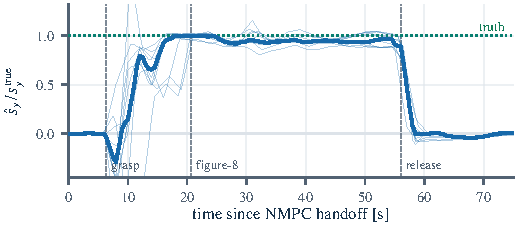
\includegraphics[width=0.92\textwidth]{Figures/fig_moment_truth.pdf}
\caption{First mass moment against ground truth (\SI{0.15}{\kg} at
\SI{2}{\meter\per\second}, $n=11$, each flight normalised by its own truth).
Truth is reconstructed offline from the simulator-measured grasp offset and never
reaches the estimator. The carry-phase estimate is biased toward zero in the
batch shown; the cause is not identified. The moment-gated detector uses the
ratio $\rho$ of \eqref{eq:rho}, which is insensitive to a common scale bias.}
\label{fig:moment}
\end{figure}

Two observations qualify the figure. First, the carry-phase estimate carries a
bias toward zero whose cause has not been identified; this is one reason the
detector is built on the ratio \eqref{eq:rho} rather than on an absolute
magnitude, since a common scale factor cancels in the ratio. Second, the $s_x$
(pitch) channel is consistently noisier than the $s_y$ (roll) channel, which
matches the torque-reconstruction correlations reported in
Section~\ref{sec:model:phys}.

Figure~\ref{fig:track3d} shows two complete missions in three dimensions,
including the two distinct post-release behaviours that
Section~\ref{sec:eval:completion} quantifies.

\begin{figure}[ht]
\centering
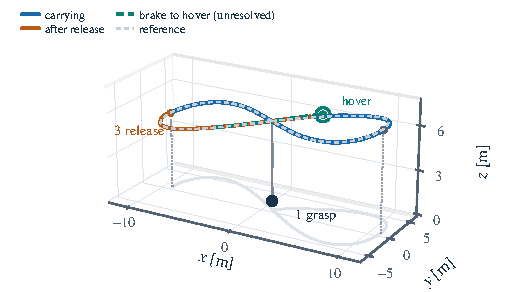
\includegraphics[width=0.92\textwidth]{Figures/fig_track_3d_measured.pdf}
\caption{Measured mission trajectory (simulator ground truth), two
\SI{0.15}{\kg}/\SI{2}{\meter\per\second} flights of the same batch: grasp, lift,
then carry along the figure-eight with \SI{\pm0.8}{\meter} vertical undulation
against the nominal reference. After the release command one flight clears the
moment vote in manoeuvre and keeps tracking; the other declares
\textsc{unresolved} at its \SI{12}{\second} timeout and brakes to hover,
confirming at \SI{16.40}{\second}. The two paths agree to within
\SI{0.12}{\meter} (median) before the timeout. Loaded tracking RMS is
\SI{0.053}{\meter} and \SI{0.060}{\meter} after release.}
\label{fig:track3d}
\end{figure}

\section{Completion and Confirmation Delay}\label{sec:eval:completion}

The complete interface confirmed release in 32 of 36 eligible flights
(Table~\ref{tab:complete}); the two-sided \SI{95}{\percent} Clopper--Pearson
interval is $[\SI{73.9}{\percent},\SI{96.9}{\percent}]$. All four failures
occurred at \SI{4}{\meter\per\second} and all four trace to estimator failure
rather than to the decision logic: three never recognised the payload and
remained \textsc{unresolved}, and one diverged after release. The pre-registered
eligibility rule would have excluded the first three and reported $31/32$; the
rule adopted here retains them.

\begin{table}[ht]
\centering
\caption{Release completion and confirmation delay, all eligible arm~B flights.
Delay runs from the release command to the end of the \SI{1.0}{\second}
confidence hold and is computed over completed flights. The two delay columns are
distinct control paths and are not pooled.}
\label{tab:complete}
\small
\begin{tabular}{@{}lcccc@{}}
\toprule
 & & & \multicolumn{2}{c}{delay median [IQR]} \\
\cmidrule(lr){4-5}
condition & $n$ & compl. & in manoeuvre & via brake-to-hover \\
\midrule
\SI{0.15}{\kg}, \SI{4}{\meter\per\second} & 11 & 10/11 & \SI{2.90}{\second} [2.90, 2.90] & \SI{16.60}{\second} [16.60, 16.60] \\
\SI{0.30}{\kg}, \SI{4}{\meter\per\second} & 13 & 10/13 & \SI{8.95}{\second} [8.00, 9.26] & \SI{16.40}{\second} [16.20, 16.70] \\
\SI{0.15}{\kg}, \SI{2}{\meter\per\second} & 12 & 12/12 & \SI{3.31}{\second} [2.95, 4.36] & \SI{16.48}{\second} [16.40, 16.50] \\
\midrule
pooled & 36 & 32/36 & \SI{3.46}{\second} [2.90, 8.00] & \SI{16.56}{\second} [16.46, 16.60] \\
\bottomrule
\end{tabular}
\\[4pt]
\footnotesize Overall delay maximum \SI{16.70}{\second}. Share confirming only
after braking to hover: \SI{50}{\percent}, \SI{40}{\percent},
\SI{50}{\percent} of completed flights by row, \SI{47}{\percent} pooled.
\end{table}

The confirmation delay is \emph{bimodal}, and the two modes correspond to the two
paths of Section~\ref{sec:frame:unresolved} rather than to a spread within one
mechanism. In 17 of the 32 completed flights the confidence crosses its threshold
while the vehicle is still flying the figure-eight, and confirmation completes in
a median of \SI{3.46}{\second}. In the remaining 15, no release evidence is
available in manoeuvre --- either $\hat\svec$ has drifted under sustained
excitation, or the frozen reference of Section~\ref{sec:frame:momentref} never
formed --- so the system reaches its \SI{12}{\second} timeout, declares
\textsc{unresolved}, brakes to hover over \SI{3}{\second}, and confirms at a
median of \SI{16.56}{\second}. Pooling the two would describe neither.

Figure~\ref{fig:mission} shows one complete in-manoeuvre confirmation.

\begin{figure}[ht]
\centering
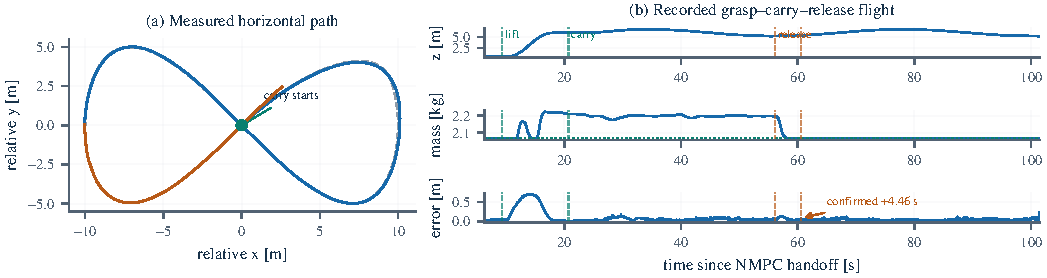
\includegraphics[width=0.96\textwidth]{Figures/fig_mission.pdf}
\caption{One eventless flight from the final batch (\SI{0.15}{\kg},
\SI{2}{\meter\per\second}). Left: measured horizontal path, coloured by carrying
and post-release phase, against the nominal reference including its amplitude
ramp. Right: height, the mass estimate actually consumed by the controller, and
the position-error norm through grasp, lift, carry, release command and
confirmation. This flight confirms in manoeuvre \SI{4.46}{\second} after the
command; it illustrates one execution and does not replace the cohort statistics
of Table~\ref{tab:complete}.}
\label{fig:mission}
\end{figure}

Table~\ref{tab:paths} records which route produced each confirmation. Every
confirmation used the controller's confidence route \eqref{eq:confirm}; the
columns record the estimator declaration, where one occurred. That three distinct
routes appear is the reason the completion rate must be read as a result for the
\emph{interface as a whole} rather than as a validation of any single detector.

\begin{table}[ht]
\centering
\caption{Confirmation paths in the 32 completed flights of
Table~\ref{tab:complete}. \emph{Moment-gated}: the detector declared before the
confidence crossed. \emph{Mass-domain}: the frozen reference never formed, the
confidence crossed during or shortly after the brake to hover, and the
mass-domain route declared \SIrange{0.9}{3.1}{\second} later. \emph{Confidence
only}: the reference never formed and no declaration occurred.}
\label{tab:paths}
\small
\begin{tabular}{@{}lcccc@{}}
\toprule
condition & $n$ & moment-gated & mass-domain & confidence only \\
\midrule
\SI{0.15}{\kg}, \SI{4}{\meter\per\second} & 10 & 9 & 1 & 0 \\
\SI{0.30}{\kg}, \SI{4}{\meter\per\second} & 10 & 1 & 3 & 6 \\
\SI{0.15}{\kg}, \SI{2}{\meter\per\second} & 12 & 9 & 0 & 3 \\
\midrule
pooled & 32 & 19 & 4 & 9 \\
\bottomrule
\end{tabular}
\end{table}

No flight in any path declared release before the command. In 23 of the 32
completed flights the presence machine made exactly two transitions, one at grasp
and one at release; in the nine confidence-only flights it never declared
\textsc{empty} within the logged window, which extended more than
\SI{40}{\second} past confirmation. Every load declaration came from sustained
mass evidence, and no external grasp signal was consumed.

\section{Does Refusing the Command Buy Anything?}\label{sec:eval:paired}

\subsection{Nominal pairs}\label{sec:eval:nominal}

Across 19 pairs in which both arms were eligible, both arms completed $19/19$
releases with no observed post-release instability
(Table~\ref{tab:paired-event}). Arm~A has zero confirmation delay by
construction. Under nominal conditions, therefore, refusing the command buys
nothing and costs a delay --- which is the correct result, since nominal
conditions are precisely those in which the command is true.

\begin{table}[ht]
\centering
\caption{Paired command-triggered ablation. Arm~A clears the model at the command
by construction; arm~B requires estimator evidence; arm~C is arm~B with its
release evidence armed only by the command. The last two rows inject a
command/physical-detachment mismatch; ``early'' means model clearing before the
joint is actually removed (``--'': not scored).}
\label{tab:paired-event}
\small
\begin{tabular}{@{}lcccc@{}}
\toprule
condition & pairs & A compl. & B compl. & early clear A/B \\
\midrule
\SI{0.15}{\kg}, \SI{4}{\meter\per\second} & 8 & 8/8 & 8/8 & -- \\
\SI{0.30}{\kg}, \SI{4}{\meter\per\second} & 3 & 3/3 & 3/3 & -- \\
\SI{0.15}{\kg}, \SI{2}{\meter\per\second} & 8 & 8/8 & 8/8 & -- \\
\midrule
nominal pooled & 19 & 19/19 & 19/19 & -- \\
\SI{0.15}{\kg}, \SI{2}{\meter\per\second} $+$ \SI{4}{\second} hold & 5 & 5/5 & 5/5 & 5/5 \ / \ 0/5 \\
\quad same, arm~C instead of A & 6 & 6/6 (C) & 6/6 & 0/6 \ / \ 0/6 \\
\bottomrule
\end{tabular}
\end{table}

Only three pairs formed at the \SI{0.30}{\kg}/\SI{4}{\meter\per\second}
condition, because arm~A crashed during or immediately after lift in 11 of 16
attempts there. That failure is a property of arm~A's gain-rewriting schedule
rather than of its release semantics: its rate scaling starts from the
lower-bound mass estimate while the box is still resting on the ground.

\subsection{Delayed detachment}\label{sec:eval:delayed}

Under a median \SI{4.01}{\second} hold between command and physical detachment,
the arms separate exactly as designed. Of twelve arm-runs one arm~A run never
armed the autopilot, leaving five valid pairs and one valid unpaired arm~B run.

In all five pairs arm~A cleared its payload model at the command, a median
\SI{4.01}{\second} before the payload actually left. Arm~B cleared before
detachment in \emph{none} of its six valid runs: it entered \textsc{unresolved}
in $5/6$ and confirmed a median \SI{12.45}{\second} after detachment, while the
remaining run confirmed \SI{3.00}{\second} after detachment. All eleven valid
runs carried an independent simulator detachment record.

The honest reading of this result is narrow. Median position-error peaks during
the hold were \SI{0.071}{\meter} for arm~A and \SI{0.068}{\meter} for arm~B, so
what the experiment demonstrates is a difference in \emph{model--plant
consistency}, not a tracking advantage and not crash avoidance. A permanently
jammed gripper --- under which arm~A would fly a loaded vehicle with an empty
model for the remainder of the mission --- was not tested.

\subsection{Command-armed confirmation and unsignaled loss}\label{sec:eval:unsignaled}

The delayed-detachment result reflects \emph{persistent confirmation}, not
eventlessness. Arm~C demonstrates this directly: armed only by the command but
otherwise identical to arm~B, it also never cleared early ($0/6$ pairs) and
confirmed sooner after detachment (median \SI{4.3}{\second} against
\SI{7.3}{\second}). If the only hazard were a slow gripper, arm~C would be the
better design.

Eventlessness earns its keep when no release command reaches the controller at
all. With such losses injected at the release phase, arm~B detected the loss in
10 of 18 paired flights --- $4/9$ at \SI{2}{\meter\per\second}, and $4/5$ and
$2/4$ at \SI{0.15}{\kg} and \SI{0.30}{\kg} at \SI{4}{\meter\per\second}, with a
median latency of \SIrange{2.2}{2.9}{\second} --- while arm~C, never armed,
detected none and carried a phantom first moment for the rest of the flight.
Seven of the eight misses occurred because the loaded moment reference had not
formed, or the payload had not been recognised, before the loss: the same
mechanism that produces the brake-to-hover mode in
Table~\ref{tab:complete}.

The cost of running a release detector throughout loaded flight --- the risk of a
false positive while the payload is still attached --- was measured and not
observed. No release was declared before a command or an injected loss in 209
loaded flights spanning \SI{3.7}{\hour}, giving a per-flight \SI{95}{\percent}
upper bound of \SI{1.4}{\percent}.

\section{Partial Payload Loss}\label{sec:eval:partial}

Losing part of a load is the case that a binary attached/detached abstraction
cannot represent at all, and it is where a continuous interface should show an
advantage in kind rather than in degree.

Pre-registered criteria were: (a) $\hat m$ enters $\pm\SI{0.02}{\kg}$ of each new
truth in at least \SI{80}{\percent} of steps; (b) the paired tracking-RMS
difference against the no-loss control arm is at most \SI{0.02}{\meter}, with no
crash; (c) no \textsc{empty} declaration after the first two losses.

At \SI{2}{\meter\per\second} all three criteria pass: the estimate followed 14 of
15 steps, with a median convergence of \SIrange{1.1}{8.8}{\second}, there was no
false \textsc{empty} declaration, and tracking was indistinguishable from the
control arm. At \SI{4}{\meter\per\second} criterion (a) reached only its
threshold ($12/15$), so recovery is claimed at \SI{2}{\meter\per\second} only.

\section{Ablations}\label{sec:eval:ablations}

\subsection{Thrust-map calibration}\label{sec:eval:thrustcal}

Section~\ref{sec:model:conline} predicted an asymmetry: the centre-of-mass
inversion is immune to the thrust coefficient because $k_f$ cancels
\eqref{eq:kfcancel}, whereas the mass channel consumes an absolute thrust and
therefore inherits the calibration error directly. The experiment confirms it,
and the sensitivity is severe.

Scaling only the estimator's thrust map by \SI{\pm5}{\percent}
(\SI{0.15}{\kg}, \SI{2}{\meter\per\second}, four repetitions per arm, 11 valid
flights) caused no pre-command release in any arm, but defeated the interface in
both directions:
\begin{itemize}
\item at $0.95$, the payload was never recognised ($0/3$) and every flight
remained \textsc{unresolved};
\item at $1.05$, a phantom \SI{+0.09}{\kg} persisted after release ($4/4$), every
flight remained \textsc{unresolved}, and one diverged;
\item at the matched value $1.00$, the payload was recognised in $4/4$.
\end{itemize}

The interpretation is that $k_f$ must be calibrated well inside \SI{5}{\percent}
for this interface to function. That is a demanding requirement, and it is the
single most important item for hardware transfer. Note also what the failure mode
is: not a wrong release, but a refusal to confirm. The interface degrades toward
\textsc{unresolved} rather than toward an empty model, which is the correct
direction for a safety-relevant decision, but it is still a failure.

\subsection{Window-balance re-initialisation}\label{sec:eval:seed}

The window vertical-force seed of \eqref{eq:winbal} replaced the instantaneous
hover approximation \eqref{eq:massseed}. A pre-registered A/B comparison at the
\SI{4}{\meter\per\second} condition gives: valid flights $10/10$ with the window
seed against $8/10$ without; figure-eight re-initialisations reduced from 29 to
1; seed error reduced from \SI{17.1}{\percent} to \SI{2.8}{\percent}; longest
consecutive re-initialisation run reduced from 17 to 1; mission completion
$10/10$ with no post-release crash.

One reservation is recorded with the result: in the enabled arm only a single
re-initialisation event occurred, so the mechanism was barely exercised there.
The reported lifecycle cohort predates this change.

\subsection{The inertia-coefficient mode}\label{sec:eval:amode}

The three alternatives to \eqref{eq:Afrozen} behave as the analysis of
Section~\ref{sec:model:Amode} predicts. In synthetic grasp--release replay, the
\textsf{coupled} mode drives the post-release mass estimate up by
\SI{53}{\percent} and holds it there; the \textsf{frozen} mode returns to
\SI{-0.34}{\percent} of the bare airframe with $\svec$ and $\dJ$ decaying
together and no bound contact. In closed loop, the \textsf{const} mode --- which
also removes the derivative, but pins the coefficient to the payload envelope ---
biases the loaded mass estimate to \SI{-3.58}{\percent} against \SI{+0.4}{\percent}
for \textsf{frozen}, and that bias was sufficient to make the mass-domain release
criterion fire prematurely, \SI{50}{\second} before the true detachment. Fixing
the derivative is necessary; fixing the \emph{value} is harmful.

\subsection{A negative result on learned stage weights}\label{sec:eval:weightlearning}

The parameterised generalisation of the retired event-triggered schedule
(Section~\ref{sec:frame:beta}) was optimised by cross-entropy search in the loop,
and the resulting schedule showed no measurable benefit over the hand-designed
rule in a paired ablation. The objective was flat over a broad neighbourhood of
that rule.

This negative result is substantively useful, and is reported rather than
omitted. What produced the benefit in the predecessor system was \emph{noticing
that the model had changed and removing stale data}; the precise magnitude of the
post-trigger weights is weakly determined by the data. A learned schedule should
therefore not be presented as a superior learned controller. It is also part of
the reason the mainline retired event logic altogether.

\section{Where the Interface Fails}\label{sec:eval:limits}

\subsection{Moment-reference formation}\label{sec:eval:refform}

The dominant failure mode is not a wrong decision but an unavailable one. In 13
of the 32 completed flights the healthy, low-dynamic, in-envelope window of
Section~\ref{sec:frame:momentref} never filled after the \textsc{loaded}
declaration, so the ratio test never ran at all. Those flights are the population
of the brake-to-hover column of Table~\ref{tab:complete} and of seven of the
eight unsignaled-loss misses.

A contributing factor was found and is smaller than the effect: the
admissibility envelope \eqref{eq:sadmissible} assumed a \SI{0.13}{\meter} grasp
offset while the gripper actually admitted \SI{0.15}{\meter}, which affected 2 of
13 \SI{0.30}{\kg} flights. It does not explain most of the missing references.
Reliable reference formation therefore remains necessary work.

A related boundary is recorded honestly: out-of-envelope $\hat\svec$ samples are
excluded from moment votes but still reach the controller's $\cvec$ through the
filter and slew limiter of \eqref{eq:lpfslew}. The exclusion protects the
decision, not the model.

\subsection{First-moment drift under sustained excitation}\label{sec:eval:drift}

Sustained figure-eight excitation can raise $\lVert\hat\svec\rVert$ from
\SI{0.012}{\kg\meter} to \SI{0.031}{\kg\meter}. Because moment evidence is then
withheld, confirmation is delayed. Deceleration restored the vote within
\SIrange{3.3}{3.4}{\second} in the affected flights, which is the mechanism
behind the brake-to-hover delays.

An online counter of envelope exceedances correlates with this outcome at
\SI{4}{\meter\per\second} --- in-manoeuvre confirmation occurred in $9/10$
flights with zero exceedances against $2/10$ otherwise, Fisher exact
$p=0.006$ --- but it misses all six delayed \SI{2}{\meter\per\second} cases, so it
is a partial diagnostic rather than a predictor. Exiting the manoeuvre earlier on
that signal is unimplemented and unvalidated.

\subsection{The operating limit}\label{sec:eval:opslimit}

\SI{0.30}{\kg} at \SI{4}{\meter\per\second} is at the vehicle's actuator limit.
Hover requires \SI{74}{\percent} of maximum thrust, but it is torque, not thrust,
that binds: in the figure-eight, pitch torque saturated within \SI{98}{\percent}
of five-second diagnostic windows and yaw within \SI{53}{\percent}
(\SI{46}{\percent} and \SI{16}{\percent} at \SI{0.15}{\kg}, at most
\SI{6}{\percent} at \SI{2}{\meter\per\second}), and the body-rate scaling of
\eqref{eq:omegascale} ran at a median $4.39$ of its cap of $5.0$. This is the
quantitative form of the feasibility boundary predicted by \eqref{eq:trimtorque}
and \eqref{eq:gain} in Chapter~\ref{ch:model}.

Three of the five arm~B pre-release crashes and three of the four incomplete
releases occurred at this condition. Every eligible \SI{2}{\meter\per\second}
flight confirmed its release. What is claimed at this limit is safe release
\emph{semantics}, not reliable flight; deployment there needs torque margin.

\subsection{Estimator failures}\label{sec:eval:estfail}

In four flights the published mass never left the empty value; in two of these,
repeated solver failures caused re-initialisation from a lower-bound seed. The
three at \SI{4}{\meter\per\second} flew without diverging and remained
\textsc{unresolved}.

One failure is more instructive than the rest. In a \SI{0.30}{\kg} flight the
estimate was unhealthy for \SI{48}{\second} before release. Because the
phase-timed release command is \emph{not} gated on estimator health, the command
was issued anyway; the frozen model no longer matched the vehicle after
detachment, and the flight diverged. Gating release on estimator health is an
obvious remedy and is not implemented.

\subsection{Configuration and default-safety}\label{sec:eval:defaults}

Every reported release batch explicitly enables the release-evidence path. Its
built-in default is \emph{off}, under which every flight ends
\textsc{unresolved}. Deployment therefore requires an explicit enable plus
startup validation of the configuration, and the implementation includes a
self-check that reports at startup which blockers, if any, would prevent the
detector from ever firing.

\subsection{Missing baselines}\label{sec:eval:missing}

The only baselines reported here are the command-triggered and command-armed arms
of Table~\ref{tab:arms}, which isolate release semantics. The evaluation does
\emph{not} include a comparison against a fixed-parameter predictive controller,
against a lumped-disturbance adaptive method such as $\mathcal{L}_1$-adaptive
NMPC \cite{hanover2021} or incremental nonlinear dynamic inversion
\cite{smeur}, or against a change-detection procedure such as CUSUM
\cite{basseville1993} applied to the same signals under a matched false-alarm
constraint. Comparison nodes for the first two exist in the implementation
(Table~\ref{tab:software}) but no frozen result set is reported for them. This is
the largest gap in the evaluation and is stated as such.

\section{Threats to Validity and Reproducibility}\label{sec:eval:validity}

All system-level evidence is software-in-the-loop. The leading threats are:

\begin{itemize}
\item \textbf{Thrust-map fidelity.} The plant generates thrust with the same
square law the estimator inverts, and rotor speeds are exact. The
\SI{\pm5}{\percent} experiment of Section~\ref{sec:eval:thrustcal} bounds one
dimension of this; speed noise, transport delay and induced inflow
\cite{bangura2012} remain untested.
\item \textbf{Clean state estimates.} The odometry available in simulation is
better than a real vehicle's, and the measurement weights \eqref{eq:Wy} are set
from representative rather than measured noise levels.
\item \textbf{Rigid attachment.} Gripper compliance and pendulum modes are not
modelled. Neither affects which signals the estimator consumes, but both would
add unmodelled dynamics to the rotational residual on which $\svec$ depends.
\item \textbf{Confounded disturbances.} A sustained vertical updraft or downdraft
is intrinsically indistinguishable from a payload change on a
collective-thrust-only residual. Wind is not evaluated in the reported cohort.
\end{itemize}

Reproducibility is handled by construction rather than by discipline. Every run
records the software revision, the resolved value of every environment switch
that affects behaviour, the problem dimensions, horizons, weights, bounds, event
timestamps, random seed and solver statistics. Runs terminated by numerical
failure remain in the denominator. The release decision used online and the one
used in offline replay are the same function, so a recorded flight can be
re-scored without re-implementing the logic.

\begin{table}[ht]
\centering
\caption{Attempts and exclusions in the paired campaign. Because the arms differ
before release, these rates are reported per arm rather than pooled, and neither
characterises end-to-end mission reliability.}
\label{tab:attempts}
\small
\begin{tabularx}{\textwidth}{@{}l c X@{}}
\toprule
\textbf{Arm} & \textbf{Attempts} & \textbf{Disposition} \\
\midrule
B (proposed) & 42 & 36 eligible; 5 crashed before the release command (three in
the \SI{0.30}{\kg}/\SI{4}{\meter\per\second} figure-eight, two during lift at
\SI{2}{\meter\per\second}); 1 did not physically attach \\
A (command-triggered) & 42 & 25 eligible; 17 pre-release crashes, 11 of them
during or just after lift at \SI{0.30}{\kg}/\SI{4}{\meter\per\second} \\
\bottomrule
\end{tabularx}
\\[4pt]
\footnotesize Table~\ref{tab:paired-event} uses the 19 pairs with both arms
eligible; Table~\ref{tab:complete} uses all 36 eligible arm~B flights; and
Table~\ref{tab:paths} uses the 32 that completed. Tail-window tracking is not
compared, because arm~B brakes to hover after an unresolved timeout while arm~A
continues the figure-eight.
\end{table}

\section{Development-Stage Evidence}\label{sec:eval:devstage}

Two earlier tests motivated the final design but used earlier code and do not
validate the deployed detector. They are reported because the design decisions
they produced are load-bearing in Chapter~\ref{ch:framework}.

First, the quantity--residual fast branch without moment evidence declared release
prematurely in 3 of 9 randomised flights during a \SI{4}{\meter\per\second}
figure-eight, the earliest \SI{51.1}{\second} before the command. This is the
observation that made moment evidence mandatory in \eqref{eq:releasedecision}.

Second, after that branch was removed, a 12-flight randomised test of the
moment-gated detector --- run before the frozen reference of
Section~\ref{sec:frame:momentref} was introduced --- produced no pre-command
declaration, 11 moment-gated releases with a median detector delay of
\SI{1.9}{\second}, and one flight that remained \textsc{unresolved}.

\end{spacing}
\newpage

%=== CHAPTER SIX ===
%% Rewritten 2026-09-18 against the deployed eventless interface.

\chapter{Conclusion and Future Work}
\label{ch:conclusion}
\begin{spacing}{1.5}
\setlength{\parskip}{0.22in}

\section{Summary}

This dissertation has treated the quadrotor payload problem as one coupled
estimation-and-control task with a specific structural difficulty at its centre.
The predictive model changes at grasp and at release in three ways: mass changes
the thrust-to-acceleration gain and the hover thrust, attachment geometry
increases roll and pitch inertia, and the horizontal centre-of-mass offset
creates a standing trim moment. Treating these as one undifferentiated
disturbance obscures that they act through different physical channels and are
identifiable to different degrees.

The structural difficulty is that the natural parameterisation of those changes
--- a payload mass together with a grasp offset --- is singular at release.
Chapter~\ref{ch:model} showed that as $\mP\to0$ the offset $\bm r_{xy}$ becomes
undefined, that holding it fixed leaves a phantom trim moment in the model, and
that the only way an optimiser can cancel that phantom is by corrupting the mass
estimate. The remedy adopted is to estimate the horizontal \emph{first mass
moment} $\svec=\mP\bm r_{xy}$ --- the product the equations of motion actually
contain --- alongside the composite mass. From that pair the centre-of-mass
offset follows as $\cvec=\svec/\mT$ with no division by the payload mass and no
knowledge of the grasp geometry, the off-diagonal inertia follows with the
payload mass cancelling exactly, and the dominant roll/pitch increment follows
from the composite mass and a weak vertical-arm prior whose error was measured to
be immaterial.

Two further reductions were necessary and were quantified rather than assumed.
The second-order horizontal inertia terms carry a factor $1/\mP$ in the new
coordinates and were discarded at a cost of \SI{2.6}{\percent} of the increment.
The remaining mass-dependent coefficient was shown to give the optimiser a lever
by which raising the mass estimate dilutes a phantom moment --- a mechanism that
drove the estimate \SI{53}{\percent} high in replay --- and was frozen within each
window to break that derivative while still tracking the true mass between
windows.

Around this model, Chapter~\ref{ch:framework} built a 16-state moving horizon
estimator driven by a wrench reconstructed from rotor speeds, a single atomic and
health-gated interface carrying that estimate to the controller, and a lifecycle
in which \emph{no attach or release notification is evidence}. The controller
issues the release command itself and does not consult it. The model is cleared
only by persistent estimator confidence; a release that cannot be confirmed
becomes \textsc{unresolved}, a hold in which the vehicle brakes smoothly to hover
and keeps waiting, rather than an assumption that the payload has gone.

In software-in-the-loop, Chapter~\ref{ch:evaluation} reported that the complete
interface confirmed release in 32 of 36 eligible flights through three distinct
confirmation paths, with median delays of \SI{3.46}{\second} in manoeuvre and
\SI{16.56}{\second} after braking to hover. Under a \SI{4}{\second} delayed
detachment, persistent confirmation avoided the early model clearing of a
command-triggered baseline in 5 of 5 pairs. The eventless interface additionally
detected 10 of 18 unsignaled payload losses that a command-armed confirmer cannot
see, at the cost of a detector exposed throughout loaded flight --- a cost that
produced no false declaration in 209 loaded flights.

\section{Principal Findings}

\begin{enumerate}
\item \textbf{The first mass moment, not the offset, is the estimable payload
geometry.} The equations of motion contain only the product. Estimating the
factors separately adds an unidentifiable direction and a singularity at exactly
the operating point of interest.

\item \textbf{Payload \emph{presence} must not be encoded in the mass channel.}
When it is, the only way for the estimator to express ``the load has gone'' is to
move the mass, which is the one quantity the controller most needs to be correct.
Augmenting $\svec$ gives presence its own channel.

\item \textbf{A parameter that appears in a denominator will be abused by an
optimiser.} Both pathologies found in this work --- the $1/\mP$ coefficient of
the discarded inertia terms, and the mass in the denominator of the ghost-moment
expression --- are instances of the same phenomenon. The fix in both cases was
structural, not a matter of tuning.

\item \textbf{An adaptive loop must be driven by a signal that is not a product
of the adaptation.} Feeding the controller's intended thrust to the estimator
makes the mass unobservable by construction; the rotor-speed reconstruction
breaks the circularity, and extending it to the yaw-reaction channel removed the
last place where the estimator could learn the controller's intent.

\item \textbf{Release evidence must come from the rotational channel.} A
collective-thrust residual cannot distinguish a payload change from a trajectory
change or a manoeuvre; a rule that omitted mandatory moment evidence released
prematurely in 3 of 9 flights, up to \SI{51}{\second} early. Making moment
collapse mandatory costs misses, which are handled as \textsc{unresolved} holds
rather than by lowering the evidence bar.

\item \textbf{A ratio needs a reference, and the reference must be formed
autonomously and then frozen.} A running maximum absorbs the very estimation
errors the detector exists to reject.

\item \textbf{Timeout is not proof.} Treating an unconfirmed release as complete
reintroduces the failure the design exists to prevent. \textsc{unresolved} is the
state that makes eventlessness deployable.

\item \textbf{Payload adaptation must update the objective as well as the state
equation.} A stale equilibrium-input baseline produces a steady-state error that
gets \emph{worse} as the input weight is increased --- a signature that
identifies the fault and that no weight tuning can remove.

\item \textbf{The interface is severely sensitive to thrust-map calibration.} A
\SI{\pm5}{\percent} error in the estimator's thrust coefficient defeated payload
recognition in both directions. This is the principal barrier to hardware
transfer, and it is a direct consequence of recovering an absolute mass from an
absolute thrust.
\end{enumerate}

\section{Limitations}

All system-level evidence is software-in-the-loop, and the simulator's plant
generates thrust with the same square law the estimator inverts. Rotor speeds are
exact; speed noise, transport delay and induced inflow are untested.

The attachment is rigid. Gripper compliance, pendulum modes, flexible and
sloshing loads are not modelled. A sustained vertical gust remains intrinsically
confounded with a payload change on a collective-thrust residual, and wind is not
evaluated.

Within the interface itself, the dominant failure is not a wrong decision but an
unavailable one: in 13 of 32 completed flights the frozen moment reference never
formed, so the ratio test never ran, and those flights are also the population of
seven of the eight unsignaled-loss misses. Out-of-envelope first-moment samples
are excluded from votes but still reach the controller's centre-of-mass parameter
through filtering. The release command is not gated on estimator health, and one
divergence is directly attributable to that omission.

The heaviest condition, \SI{0.30}{\kg} at \SI{4}{\meter\per\second}, sits at the
vehicle's torque limit rather than at an operating point: pitch torque saturated
within \SI{98}{\percent} of diagnostic windows there. Safe release
\emph{semantics} are claimed at that limit; reliable flight is not.

Finally, the baseline set is thin. The reported comparisons isolate release
semantics only. No comparison against a fixed-parameter controller, a
lumped-disturbance adaptive controller, or a formal change-detection procedure
under a matched false-alarm constraint is included, although implementations of
the first two exist in the codebase.

\section{Future Work}

\paragraph{Reference formation.} The single highest-value improvement is to make
the loaded moment reference form reliably. Roughly \SI{40}{\percent} of flights
never produced one, and that single deficiency accounts for the brake-to-hover
delay mode, most unsignaled-loss misses, and the confidence-only confirmations.
Candidates include forming the reference during the lift transient rather than
requiring a later quiet window, admitting a direction-only reference when the
magnitude is unstable, and exiting the manoeuvre early on the envelope-exceedance
counter that already correlates with the outcome at \SI{4}{\meter\per\second}.

\paragraph{Calibration robustness.} Because the mass channel consumes an absolute
thrust, its accuracy is bounded by the accuracy of $k_f$. Two directions are
open: propagating a calibration uncertainty into the estimator weights so that
the interface degrades gracefully rather than at a threshold, and exploiting the
\emph{calibration-invariant} structure already present in the centre-of-mass
inversion, in which $k_f$ cancels, as an independent cross-check on the mass
channel.

\paragraph{Health-gated release.} The release command should not be issued while
the estimator is unhealthy. This is a small change with a demonstrated failure
behind it.

\paragraph{Baselines and detection theory.} A matched-false-alarm comparison
against CUSUM and related procedures on the same signals would establish whether
the hand-built persistence rules are near the achievable operating curve or far
from it. A comparison against a fixed-parameter and an $\mathcal{L}_1$-adaptive
controller would separate the benefit of the payload model from the benefit of
adaptation in general.

\paragraph{Modelling extensions.} The yaw inertia increment and the second-order
horizontal terms could be restored if a formulation is found that avoids the
$1/\mP$ degeneracy --- for example by regularising the payload mass away from
zero only inside those terms. A random-walk treatment of the payload states would
remove the remaining one-window transient, provided the Hessian scaling problem
it caused can be solved.

\paragraph{Hardware transfer.} Transfer should proceed in stages: motor-stand
calibration of $k_f$ and $k_m$ against measured thrust and reaction torque;
tethered hover with the estimator running open-loop; centred payload pickup;
eccentric pickup; and only then dynamic flight. Simulated rotor speeds must be
replaced by electronic-speed-controller telemetry, and the noise, delay and
quantisation of that telemetry re-measured rather than assumed. A supervisor
monitoring solver status, estimator health and input margin should gate every
stage.

\section{Closing Remark}

The lesson that generalises beyond this vehicle is about the relationship between
an estimate and a decision. Online estimation is useful only when the estimated
quantity enters the controller in a physically and numerically consistent way ---
and a system that acts on events it has been \emph{told} about, rather than on
what it can \emph{observe}, has no way to notice when the two disagree. Choosing
a parameterisation that stays well posed through the transition, and refusing to
let a command stand in for evidence, are the two decisions that made the rest of
this architecture work.

\end{spacing}
\newpage

%==== ENDING PART ===

\renewcommand\bibname{References}
\bibliographystyle{unsrt}
\begin{spacing}{1.5}
\bibliography{Ref/References}
\end{spacing}
\newpage

%=== APPENDICES ===
\begin{appendices}
\label{cha:appendices}

\chapter{Implemented Optimal Control Problem Configuration}
\markboth{Appendix A}{}

\begin{spacing}{1.5}

\begin{table}[ht]
\centering
\caption{NMPC configuration (deployed default).}
\begin{tabular}{@{}ll@{}}
\toprule
State dimension & 13 \\
Input dimension & 4 \\
Runtime parameter dimension & 23 \\
Prediction stages & $N=20$ \\
Sampling interval & $\Delta t=\SI{0.05}{\second}$ \\
Prediction horizon & \SI{1.0}{\second} \\
Solve rate & \SI{20}{\hertz}; setpoints published at \SI{50}{\hertz} \\
Integrator & Explicit RK4 \\
NLP method & Full SQP with merit backtracking \\
QP solver & Partial-condensing HPIPM \\
Hessian & Gauss--Newton \\
Thrust box & $[\SI{1.27}{\newton},\ \SI{31.35}{\newton}]$ (actuator envelope) \\
Torque box & $\pm\SI{0.5}{\newton\meter}$ roll/pitch, $\pm\SI{0.2}{\newton\meter}$ yaw \\
Bryson tolerances (state) & $0.1$\,m, $0.3$\,m/s, $0.05$, $0.3$\,rad/s \\
Bryson tolerances (input) & $2.0$\,N, $0.5$\,N\,m, $0.2$\,N\,m \\
Terminal scaling & $20\times$ position, $1\times$ velocity, $2\times$ attitude, $0.2\times$ rate \\
\bottomrule
\end{tabular}
\end{table}

\begin{table}[ht]
\centering
\caption{MHE configuration (deployed default). The prior-free column lists the
values taken by the ablation of Section~\ref{sec:frame:weights}.}
\small
\begin{tabularx}{\textwidth}{@{}p{0.34\textwidth} X X@{}}
\toprule
 & \textbf{Deployed} & \textbf{Prior-free ablation} \\
\midrule
Augmented state dimension & 16 ($x$, $\mT$, $s_x$, $s_y$) & same \\
Process-noise dimension & 13 (physical states only) & same \\
Runtime parameter dimension & 7 (wrench, previous $\hat m$, $r_z$) & same \\
Estimation stages / interval & $N=20$ / \SI{0.1}{\second} & same \\
Moving horizon & \SI{2.0}{\second} & same \\
Mass box & $[0.95\,\mB,\ \SI{5.0}{\kg}]$ & $[\SI{0.2}{\kg},\ \SI{5.0}{\kg}]$ \\
Mass arrival $\sigma$ & \SI{3.16}{\kg} & \SI{1000}{\kg} \\
First-moment box & $|s_i|\le\SI{1.5}{\kg\meter}$ & same \\
First-moment arrival $\sigma$ & \SI{0.1}{\kg\meter} & same \\
Initial iterate & window force balance \eqref{eq:winbal} & same \\
Inertia coefficient $A$ & lagged, \eqref{eq:Afrozen}; switch value \texttt{frozen} & same \\
Vertical-arm prior $r_z$ & \SI{-0.47}{\meter} & same \\
Stage weighting $\beta_j$ & $\equiv 1$ (event logic retired) & same \\
Re-anchor trigger & 5 consecutive solver failures & same \\
Output filter & first order, $\tau=\SI{0.25}{\second}$ & same \\
NLP / QP method & Full SQP / partial-condensing HPIPM & same \\
\bottomrule
\end{tabularx}
\end{table}

\begin{table}[ht]
\centering
\caption{Payload interface and lifecycle settings.}
\small
\begin{tabularx}{\textwidth}{@{}p{0.40\textwidth} X@{}}
\toprule
Frame fields & $\mT$, $\svec$, $\cvec$, $\dJ_{\mathrm{diag}}$, $J_{\mathrm{diag}}$, $\gamma$, health, solution age \\
Input freshness / solution freshness & \SI{0.30}{\second} / \SI{0.30}{\second} \\
Consumer receive-age limit & \SI{0.35}{\second} \\
Controller-side filter $\tau$ & \SI{0.20}{\second} \\
Slew limits ($\mT$ / $\svec$ / $\dJ$) & $0.60$\,kg/s / $0.080$\,kg\,m/s / $0.080$\,kg\,m$^2$/s \\
Confidence thresholds ($\mP$, $\lVert\svec\rVert$, $\dJ_{xy}$) & $(0.015,0.060)$, $(0.0015,0.0060)$, $(0.0020,0.0100)$ \\
Confirmation & $\gamma>0.90$ held \SI{1.0}{\second} \\
Moment-collapse ratio / sanity bound & $\rho<0.30$ / $\lVert\svec\rVert<\SI{0.008}{\kg\meter}$ \\
Quantity-empty threshold / persistence & $\mP<\SI{0.030}{\kg}$ / 5 frames (slow path) \\
Residual half-window / floor / persistence & \SI{0.3}{\second} / \SI{0.9}{\newton} / 2 (normal), 4 (strong) \\
Residual evidence validity & \SI{3.0}{\second} \\
Reference window & 20 frames; $\lVert\bm\omega\rVert\le0.15$, $\lVert\bm v_{xy}\rVert\le0.20$ \\
Reference admissibility & $\lVert\svec\rVert\le\SI{0.039}{\kg\meter}$ \\
Reference statistics & CV $\le0.25$; direction $\ge0.90$; \SI{20}{\percent}-trimmed mean \\
\textsc{unresolved} timeout / brake duration & \SI{12}{\second} / \SI{3}{\second} \\
Body-rate scale cap / dead band & $5.0$ / $0.08$ \\
Body-rate scale $\tau$ / rise / recover & \SI{0.5}{\second} / $4.0$\,s$^{-1}$ / $1.5$\,s$^{-1}$ \\
Body-rate headroom fraction / hard limit & $0.95$ / \SI{2.0}{\radian\per\second} \\
Attach inertia bootstrap & envelope \SI{0.30}{\kg}; confirm \SI{0.5}{\second}; fade \SI{0.5}{\second} \\
\bottomrule
\end{tabularx}
\end{table}
\end{spacing}

\clearpage
\chapter{Experiment Record Template}
\markboth{Appendix B}{}

\begin{spacing}{1.5}
Each run stores the following metadata with its log, so that any reported figure
can be regenerated from retained data:
\begin{enumerate}
\item repository revision, build timestamp and generated-solver identity;
\item the \emph{resolved value} of every environment switch that affects
behaviour --- not only those explicitly set, since a default that is never
written to disk is the commonest way for a batch to become unattributable;
\item airframe mass and inertia calibration, rotor coefficients and the fixed
actuator limits;
\item payload mass and attachment geometry for offline scoring, together with
evidence that neither reached the adaptive path;
\item trajectory parameters, grasp and release phase, and random seed;
\item both horizons, weights, bounds and solver options;
\item topic rates and measured end-to-end latency;
\item the complete lifecycle event trace, with timestamps for every state
transition and every release vote;
\item termination reason, solver status sequence and constraint activity.
\end{enumerate}

Results tables carry one row per run in the retained data, not only an aggregate,
so that failed runs cannot disappear during manual selection. Runs terminated by
numerical failure remain in the denominator; any manual exclusion must name a
pre-declared logging or infrastructure fault.
\end{spacing}

\clearpage
\chapter{Pre-Submission Checklist}
\markboth{Appendix C}{}

\begin{spacing}{1.5}
\begin{enumerate}
\item Replace the candidate, programme, supervisor and acknowledgement
placeholders in \texttt{main.tex} and the front matter.
\item Confirm the declaration statements against the current NTU MAE wording.
\item Set \texttt{\string\showdraftnotesfalse} in \texttt{main.tex}.
\item Verify every numerical claim in Chapter~\ref{ch:evaluation} against a
retained log or analysis script, and confirm that no reported batch mixes
configurations.
\item Confirm that no run in any reported batch passes payload truth, a
task-specific payload mass, or an attach/release notification into the adaptive
path, and that the platform envelope is the only mass-valued constant remaining.
\item State, for each reported arm, which release baseline setting was active.
\item Run BibTeX and recompile until all cross-references resolve.
\item Check the final PDF against the current NTU MAE formatting checklist.
\end{enumerate}
\end{spacing}

\end{appendices}

%==== END OF ALL ===
\end{document}
